\chapter{Appendix Part II}
\section{Definitions}
\subsection{Definition of the normalized Shannon Index}\label{sec:definition_shannon_index}
We calculate the normalized Shannon index as follows:
\begin{equation}
	- \frac{1}{\log_2(|C|)} \cdot \nsum_{i \in C} \frac{n_i}{n} \cdot \log_2 (\frac{n_i}{n})
\end{equation}
where $n$ is the total number of samples of the dataset, $C$ is the set of all classes, and $n_i$ is the number of samples of the class $i \in C$. As an example, for the dataset \textsc{Proteins} the variables are set to be the following: $C = \{0, 1\}$ with $n_0 = 663$ and $n_1 = 450$, so that $n = 1113$, yielding a rounded value of $0.973$.

\subsection{Theoretical Maximum Accuracy Analysis}

\begin{table}[H]
	\caption{An overview of the maximum theoretical classification accuracy achievable for each dataset based on the number of 1-WL iterations in percent. A hyphen ``-'' indicates that the maximum accuracy has converged with fewer iterations, implying that further iterations do not improve the accuracy. ``\textsc{Oom}'' denotes out of memory error.}
    \centering
	\label{tab:max_accuracies_app}
	\begin{tabular}{@{}c <{\enspace}@{}lcccccc@{}}	\toprule
			& \multirow{3}{*}{\vspace*{4pt}\textbf{Datasets}}&\multicolumn{6}{c}{\textbf{Iterations of the \wl algorithm}}\\\cmidrule{3-8}
			& & {0}  & {1}  & {2}  & {3} & {4}  & {5}
			\\
			\toprule

			\multirow{4}{*}{\rotatebox{90}{Bioinformatics}}
            & DD &1.00 & - & - & - & - & - \\
            & ENZYMES &0.81 & 1.00 & - & - & - & - \\
            & KKI & 1.00 & - & - & - & - & - \\
            & OHSU & 1.00 & - & - & - & - & - \\
            & Peking\_1 & 1.00 & - & - & - & - & - \\
            & PROTEINS &0.92 & 1.00 & - & - & - & -\\

            \cmidrule{2-8}
            \multirow{9}{*}{\rotatebox{90}{Small molecules}}
            & AIDS & 1.00 & 1.00 & - & - & - & - \\
            & BZR & 0.96 & 0.99 & 1.00 & - & - & - \\
            & COX2 & 0.93 & 0.96 & 0.99 & 1.00 & - & - \\
            & DHFR & 0.92 & 0.95 & 1.00 & 1.00 & - & - \\
            & FRANKENSTEIN & 0.63 & 0.77 & 0.88 & 0.89 & 0.89 & - \\
            & MUTAG &0.93 & 0.96 & 0.99 & 1.00 & - & - \\
            & NCI1 &0.91 & 1.00 & 1.00 & 1.00 & - & - \\
            & NCI109 & 0.92 & 1.00 & 1.00 & 1.00 & - & - \\
            & PTC\_MR &0.92 & 0.98 & 0.99 & - & - & - \\
            \cmidrule{2-8}

            \multirow{6}{*}{\rotatebox{90}{Social networks}}
            & COLLAB &0.61 & 0.98 & - & - & - & - \\
            & IMDB-BINARY &0.61 & 0.89 & - & - & - & - \\
            & IMDB-MULTI &0.44 & 0.63 & - & - & - & - \\
            & REDDIT-BINARY &0.84 & 1.00 & - & - & - & - \\
            & REDDIT-MULTI-5K & 0.55 & 1.00 & - & - & - & - \\
            & REDDIT-MULTI-12K & 0.36 & \textsc{Oom} & \textsc{Oom} & \textsc{Oom} & \textsc{Oom} & \textsc{Oom} \\
			\bottomrule
		\end{tabular}             
\end{table}

\subsection{Hyperparameter Configuration and Optimization}

\begin{table}[H]
	\caption{\wlnn!}
	\label{tab:sweep_wlnn}
    \resizebox{.975\textwidth}{!}{ 	\renewcommand{\arraystretch}{0.9}
		\begin{tabular}{@{}c <{\enspace}@{}lcccccc@{}}	\toprule
			& \multirow{3}{*}{\vspace*{4pt}\textbf{Hyperparameter}}&\multicolumn{6}{c}{\textbf{Dataset}}\\\cmidrule{3-8}
			& & {\textsc{Enzymes}}         &  {\textsc{Imdb-Binary}}  & {\textsc{Mutag}}           & {\textsc{NCI1}}       & {\textsc{Proteins}}  & {\textsc{Reddit-Binary}}
			\\
			\toprule
			\multirow{6}{*}{}            
            & Batch Size & 32 & 32 & 32 & 33 & 32 & 32\\
            & Learning Rate & $X \sim \textit{U}(0.0001, 0.1)$ & $X \sim \textit{U}(0.0001, 0.1)$ & $X \sim \textit{U}(0.0001, 0.1)$ & $X \sim \textit{U}(0.0001, 0.1)$ & $X \sim \textit{U}(0.0001, 0.1)$ & $X \sim \textit{U}(0.0001, 0.1)$ \\
            & Max Epochs & 200 & 200 & 200 & 200 & 200 & 200 \\
            & Optimizer & Adam & Adam & Adam & Adam & Adam & Adam \\
            & Scheduler & ReduceLROnPlateau & ReduceLROnPlateau & ReduceLROnPlateau & ReduceLROnPlateau & ReduceLROnPlateau & ReduceLROnPlateau \\
            \midrule
			& Number of \wl iterations & $\{1, 2, 3\}$ & $\{1, 2, 3, 4\}$ & $\{1, 2, 3, 4\}$ & $\{1, 2, 3\}$ & $\{1, 2, 3, 4\}$ & $\{1, 2\}$ \\
            & Use \wl-Convergence & False & False & False & False & False & False \\
            \midrule
            & \mlp Activation Function & ReLU & ReLU & ReLU & ReLU & ReLU & ReLU \\
            & \mlp Normalization & BatchNorm & BatchNorm & BatchNorm & BatchNorm & BatchNorm & BatchNorm \\ 
            & \mlp Number of Layers & $\{2, 3, 4, 5\}$ & $\{2, 3, 4, 5\}$ & $\{2, 3, 4, 5\}$ & $\{2, 3, 4, 5\}$ & $\{2, 3, 4, 5\}$ & $\{2, 3, 4, 5\}$ \\
            & \mlp Dropout & $X \sim \textit{U}(0, 0.2)$ & $X \sim \textit{U}(0, 0.2)$ & $X \sim \textit{U}(0, 0.2)$ & $X \sim \textit{U}(0, 0.2)$ & $X \sim \textit{U}(0, 0.2)$ & $X \sim \textit{U}(0, 0.2)$ \\
            \midrule
            & Embedding Dimension & $\{\text{None}, 16, 32, 64, 128\}$ & $\{\text{None}, 16, 32, 64, 128\}$ & $\{\text{None}, 16, 32, 64, 128\}$ & $\{\text{None}, 16, 32, 64, 128\}$ & $\{\text{None}, 16, 32, 64, 128\}$ & $\{\text{None}, 16, 32, 64, 128\}$ \\
            & Pooling function & $\{\textsf{Max}, \textsf{Mean}, \textsf{Sum}\}$ & $\{\textsf{Max}, \textsf{Mean}, \textsf{Sum}\}$ & $\{\textsf{Max}, \textsf{Mean}, \textsf{Sum}\}$ & $\{\textsf{Max}, \textsf{Mean}, \textsf{Sum}\}$ & $\{\textsf{Max}, \textsf{Mean}, \textsf{Sum}\}$ & $\{\textsf{Max}, \textsf{Mean}, \textsf{Sum}\}$\\
			\bottomrule
		\end{tabular}}              
\end{table}

\begin{table}[H]
	\caption{An Overview of hyperparameters we sweeped and tested each dataset with.}
	\label{tab:sweep_gnn}
    \resizebox{.975\textwidth}{!}{ 	\renewcommand{\arraystretch}{0.9}
		\begin{tabular}{@{}c <{\enspace}@{}lcccccc@{}}	\toprule
			& \multirow{3}{*}{\vspace*{4pt}\textbf{Hyperparameter}}&\multicolumn{6}{c}{\textbf{Dataset}}\\\cmidrule{3-8}
			& & {\textsc{Enzymes}}         &  {\textsc{Imdb-Binary}}  & {\textsc{Mutag}}           & {\textsc{NCI1}}       & {\textsc{Proteins}}  & {\textsc{Reddit-Binary}}
			\\
			\toprule
			\multirow{6}{*}{}            
            & Batch Size & 32 & 32 & 32 & $\{33, 129\}$ & 32 & 32\\
            & Learning Rate & $X \sim \textit{U}(0.0001, 0.1)$ & $X \sim \textit{U}(0.0001, 0.1)$ & $X \sim \textit{U}(0.0001, 0.1)$ & $X \sim \textit{U}(0.0001, 0.1)$ & $X \sim \textit{U}(0.0001, 0.1)$ & $X \sim \textit{U}(0.0001, 0.1)$ \\
            & Max Epochs & 200 & 200 & 200 & 200 & 200 & 200 \\
            & Optimizer & Adam & Adam & Adam & Adam & Adam & Adam \\
            & Scheduler & ReduceLROnPlateau & ReduceLROnPlateau & ReduceLROnPlateau & ReduceLROnPlateau & ReduceLROnPlateau & ReduceLROnPlateau \\
            \midrule
            & GNN Architecture & $\{\gat, \gcn, \gin\}$ & $\{\gat, \gcn, \gin\}$ & $\{\gat, \gcn, \gin\}$ & $\{\gat, \gcn, \gin\}$ & $\{\gat, \gcn, \gin\}$ & $\{\gat, \gcn, \gin\}$ \\
            & GNN Activation Function & ReLU & ReLU & ReLU & ReLU & ReLU & ReLU \\
            & GNN Dropout & $X \sim \textit{U}(0, 0.2)$ & $X \sim \textit{U}(0, 0.2)$ & $X \sim \textit{U}(0, 0.2)$ & $X \sim \textit{U}(0, 0.2)$ & $X \sim \textit{U}(0, 0.2)$ & $X \sim \textit{U}(0, 0.2)$ \\
            & GNN Hidden Dimension & $\{16, 32, 64, 128\}$ & $\{16, 32, 64, 128\}$ & $\{16, 32, 64, 128\}$ & $\{16, 32, 64, 128\}$ & $\{16, 32, 64, 128\}$ & $\{16, 32, 64, 128\}$ \\
            & GNN Jumping-Knowledge & cat & cat & cat & cat & cat & cat \\
            & GNN Number of Layers & $5$ & $5$ & $5$ & $5$ & $5$ & $5$ \\
            \midrule
            & \mlp Activation Function & ReLU & ReLU & ReLU & ReLU & ReLU & ReLU \\
            & \mlp Normalization & BatchNorm & BatchNorm & BatchNorm & BatchNorm & BatchNorm & BatchNorm \\ 
            & \mlp Number of Layers & $\{2, 3, 4, 5\}$ & $\{2, 3, 4, 5\}$ & $\{2, 3, 4, 5\}$ & $\{2, 3, 4, 5\}$ & $\{2, 3, 4, 5\}$ & $\{2, 3, 4, 5\}$ \\
            & \mlp Dropout & $X \sim \textit{U}(0, 0.2)$ & $X \sim \textit{U}(0, 0.2)$ & $X \sim \textit{U}(0, 0.2)$ & $X \sim \textit{U}(0, 0.2)$ & $X \sim \textit{U}(0, 0.2)$ & $X \sim \textit{U}(0, 0.2)$ \\
            \midrule
            & Pooling function & $\{\textsf{Max}, \textsf{Mean}, \textsf{Sum}\}$ & $\{\textsf{Max}, \textsf{Mean}, \textsf{Sum}\}$ & $\{\textsf{Max}, \textsf{Mean}, \textsf{Sum}\}$ & $\{\textsf{Max}, \textsf{Mean}, \textsf{Sum}\}$ & $\{\textsf{Max}, \textsf{Mean}, \textsf{Sum}\}$ & $\{\textsf{Max}, \textsf{Mean}, \textsf{Sum}\}$\\
			\bottomrule
		\end{tabular}}              
\end{table}

\begin{table}[H]
	\caption{\wlnn!}
	\label{tab:sweep_wlnn_reg}
    \resizebox{.975\textwidth}{!}{ 	\renewcommand{\arraystretch}{0.9}
		\begin{tabular}{@{}c <{\enspace}@{}lcccc@{}}	\toprule
			& \multirow{3}{*}{\vspace*{4pt}\textbf{Hyperparameter}}&\multicolumn{4}{c}{\textbf{Dataset}}\\\cmidrule{3-6}
			& & {\textsc{Alchemy}}         &  {\textsc{Alchemy(10k)}}  & {\textsc{Zinc}}           & {\textsc{Zinc(10k)}}
			\\
			\toprule
			\multirow{6}{*}{}            
            & Batch Size & 25 & 25 & 25 & 25\\
            & Learning Rate & 0.001 & 0.001 & 0.001 & 0.001 \\
            & Max Epochs & 1000 & 1000 & 1000 & 1000 \\
            & Optimizer & Adam & Adam & Adam & Adam \\
            & Scheduler & ReduceLROnPlateau & ReduceLROnPlateau & ReduceLROnPlateau & ReduceLROnPlateau \\
            \midrule
			& Number of \wl iterations & $\{1, 2, 3\}$ & $\{1, 2, 3, 4\}$ & $\{1, 2, 3\}$ & $\{1, 2, 3, 4\}$\\
            & Use \wl-Convergence & False & False & False & False \\
            \midrule
            & \mlp Activation Function & ReLU & ReLU & ReLU & ReLU\\
            & \mlp Normalization & BatchNorm & BatchNorm & BatchNorm & BatchNorm\\ 
            & \mlp Number of Layers & $\{2, 3, 4, 5\}$ & $\{2, 3, 4, 5\}$ & $\{2, 3, 4, 5\}$ & $\{2, 3, 4, 5\}$\\
            & \mlp Dropout & $X \sim \textit{U}(0, 0.2)$ & $X \sim \textit{U}(0, 0.2)$ & $X \sim \textit{U}(0, 0.2)$ & $X \sim \textit{U}(0, 0.2)$\\
            \midrule
            & Embedding Dimension & $\{\text{None}, 16, 32, 64, 128\}$ & $\{\text{None}, 16, 32, 64, 128\}$ & $\{\text{None}, 16, 32, 64, 128\}$ & $\{\text{None}, 16, 32, 64, 128\}$\\
            & Pooling function & $\{\textsf{Max}, \textsf{Mean}, \textsf{Sum}\}$ & $\{\textsf{Max}, \textsf{Mean}, \textsf{Sum}\}$ & $\{\textsf{Max}, \textsf{Mean}, \textsf{Sum}\}$ & $\{\textsf{Max}, \textsf{Mean}, \textsf{Sum}\}$\\
			\bottomrule
		\end{tabular}}              
\end{table}

\section{Analysis}

\begin{table}[H]
    \caption{Overview of the number of unique colors in the colorings computed by the \wl algorithm when applied to each dataset. Specifically, we specified the number of iterations of the \wl algorithm. Additionally, the ``\# Nodes'' column showcases the maximum number of unique colors that can be appear in the colorings.}
    \label{tab:unique_colors}
    \centering
    \resizebox{.975\textwidth}{!}{ 	\renewcommand{\arraystretch}{0.9}
    \begin{tabular}{lrrrrrrrrrrr | r}
    \toprule
        \multirow{3}{*}{\vspace*{4pt}\textbf{Dataset}}&\multicolumn{11}{c}{\textbf{Number of \wl Iterations}}\\\cmidrule{2-13}
        & 0 & 1 & 2 & 3 & 4 & 5 & 6 & 7 & 8 & 9 & 10 & \# Nodes\\
        \midrule
        {\textsc{Enzymes}}  & 2 & 231 & 10\,416 & 15\,208 & 16\,029 & 16\,450 & 16\,722 & 16\,895 & 17\,026 & 17\,130 & 17\,204 & 195\,80\\
        {\textsc{Imdb-Binary}} & 1 & 65 & 2\,931 & 3\,595 & 3\,595 & 3\,595 & 3\,595 & 3\,595 & 3\,595 & 3\,595 & 3\,595 & 19\,773 \\
        {\textsc{Mutag}}  & 2 & 33 & 174 & 572 & 1\,197 & 1\,766 & 2\,167 & 2\,403 & 2\,511 & 2\,560 & 2\,579 & 3\,371 \\
        {\textsc{NCI1}} & 2 & 292 & 4\,058 & 22\,948 & 44\,508 & 58\,948 & 68\,632 & 75\,754 & 81\,263 & 85\,590 & 88\,968 & 122\,747\\
        {\textsc{Proteins}} & 2 & 297 & 20\,962 & 35\,676 & 37\,940 & 38\,653 & 38\,926 & 39\,064 & 39\,141 & 39\,180 & 39\,203 & 43\,471\\
        {\textsc{Reddit-Binary}} & 1 & 566 & 71\,893 & 244\,529 & 317\,728 & 333\,258 & 335\,961 & 336\,412 & 336\,490 & 336\,506 & 336\,507 & 859\,254 \\
        \bottomrule
    \end{tabular}}
\end{table}


\section{Visualization of the Approximation Performance of GNNs}
\begin{figure}[!ht]
    \centering
    \begin{minipage}[b]{0.45992852703\textwidth}
        \centering
        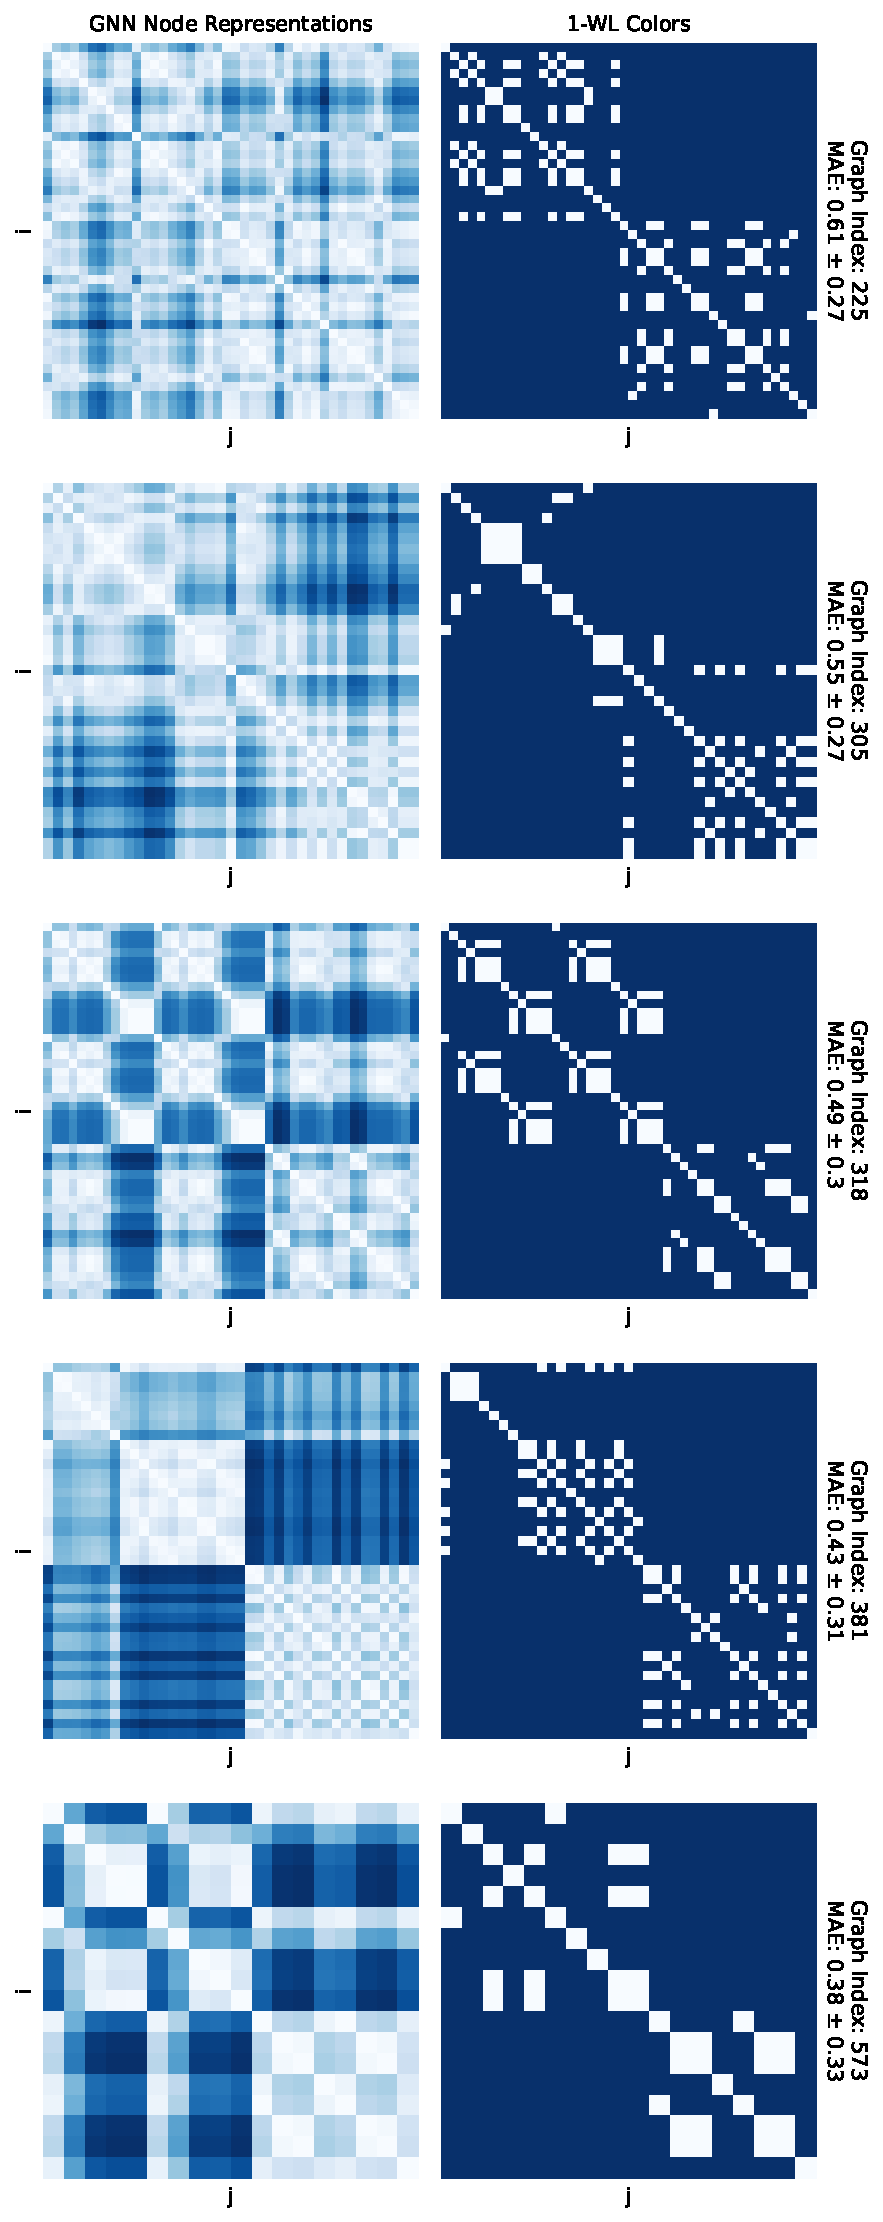
\includegraphics[width=\textwidth, left]{Figures/heatmaps_ENZYMES_0.pdf}
    \end{minipage}
    \hfill
    \begin{minipage}[b]{0.53007147296\textwidth}
        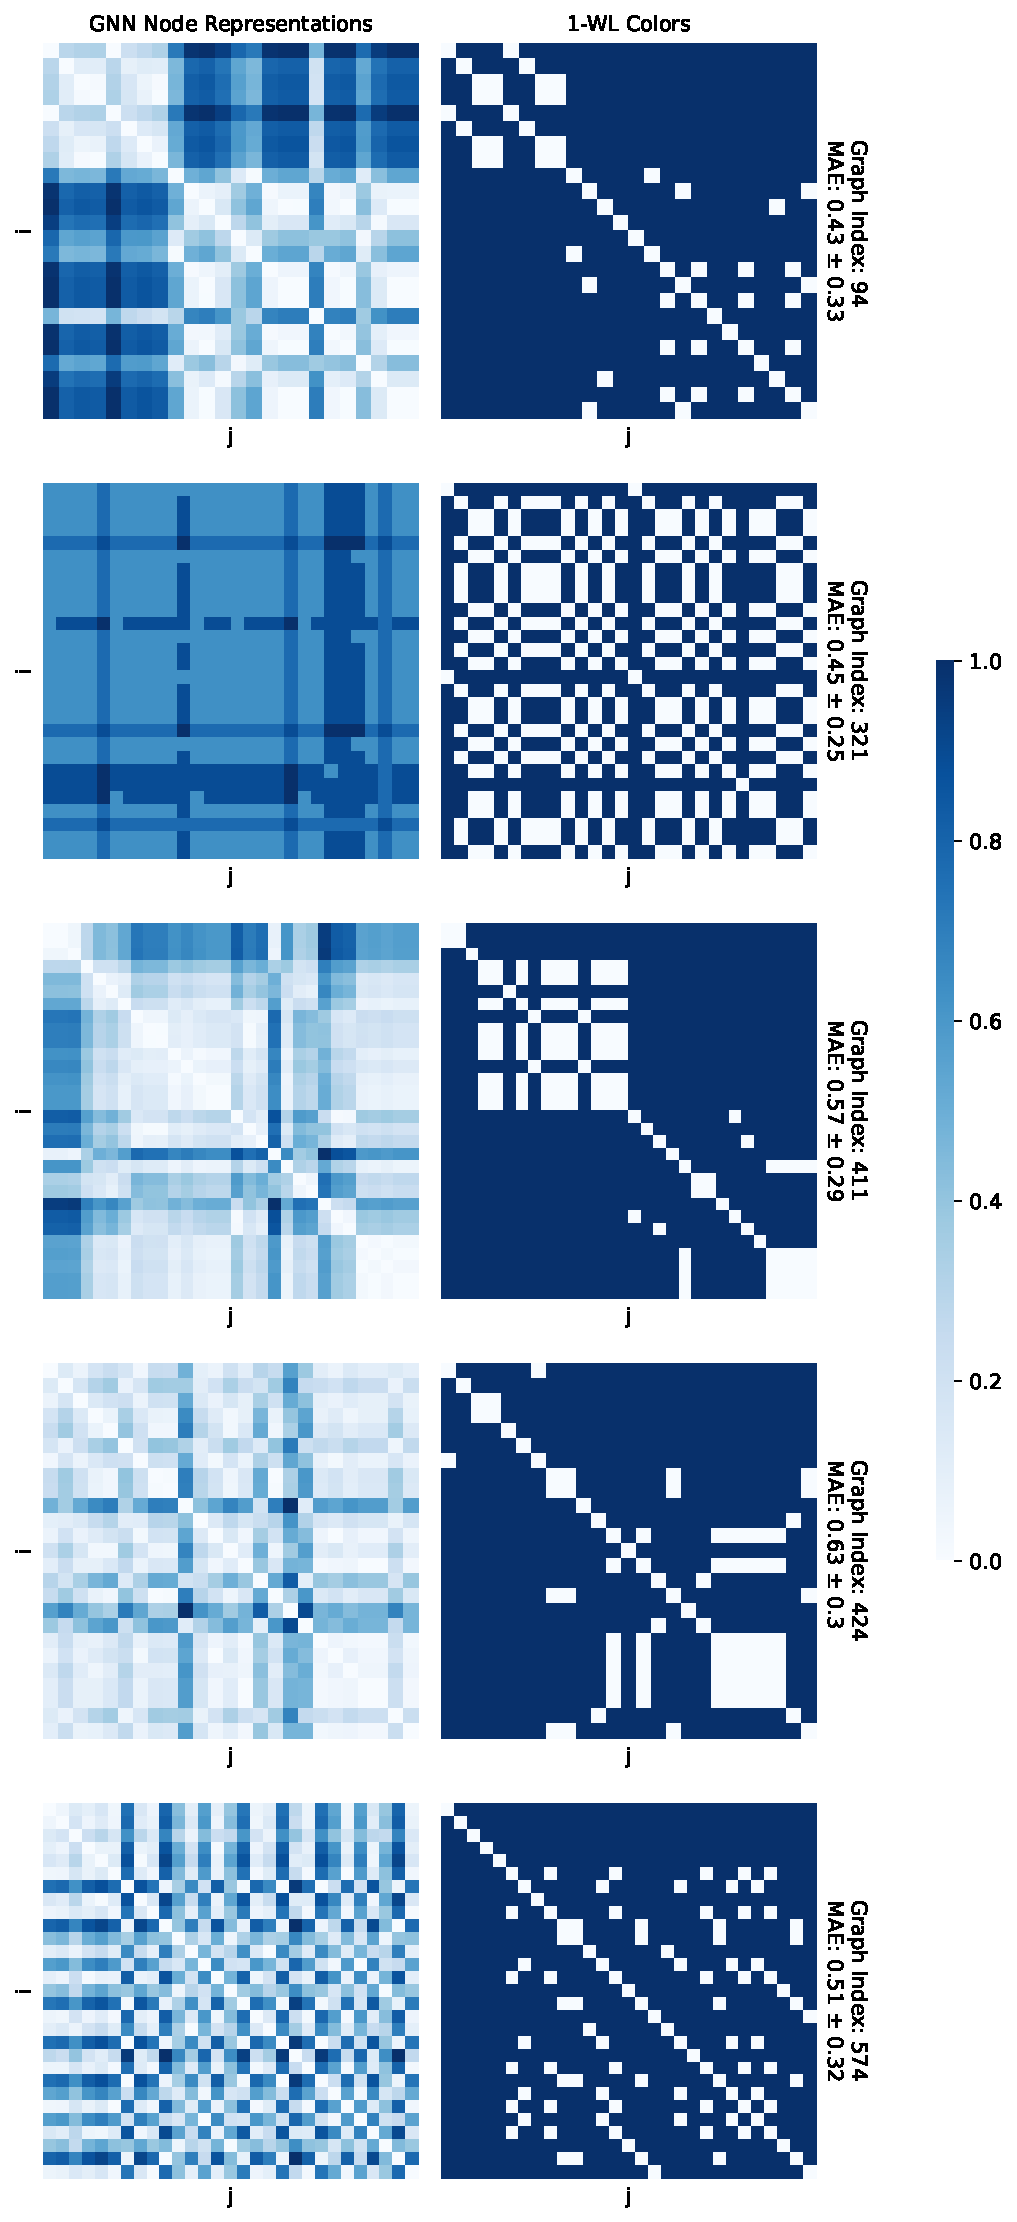
\includegraphics[width=\textwidth, right]{Figures/heatmaps_ENZYMES_1.pdf}
    \end{minipage}
    \hfill
    \caption{Visualizing the performance of the best performing GNN on the \textsc{Enzymes} dataset in approximating node colors computed by the 1-WL algorithm. The ten graphs shown are randomly sampled from the GNN's test set, and the 1-WL algorithm ran only for one iteration. The average error for the entire test set is $0.49 \pm 0.3$.}
    \label{fig:gnn_approx_enzymes}
\end{figure}

\begin{figure}[!ht]
    \centering
    \begin{minipage}[b]{0.45992852703\textwidth}
        \centering
        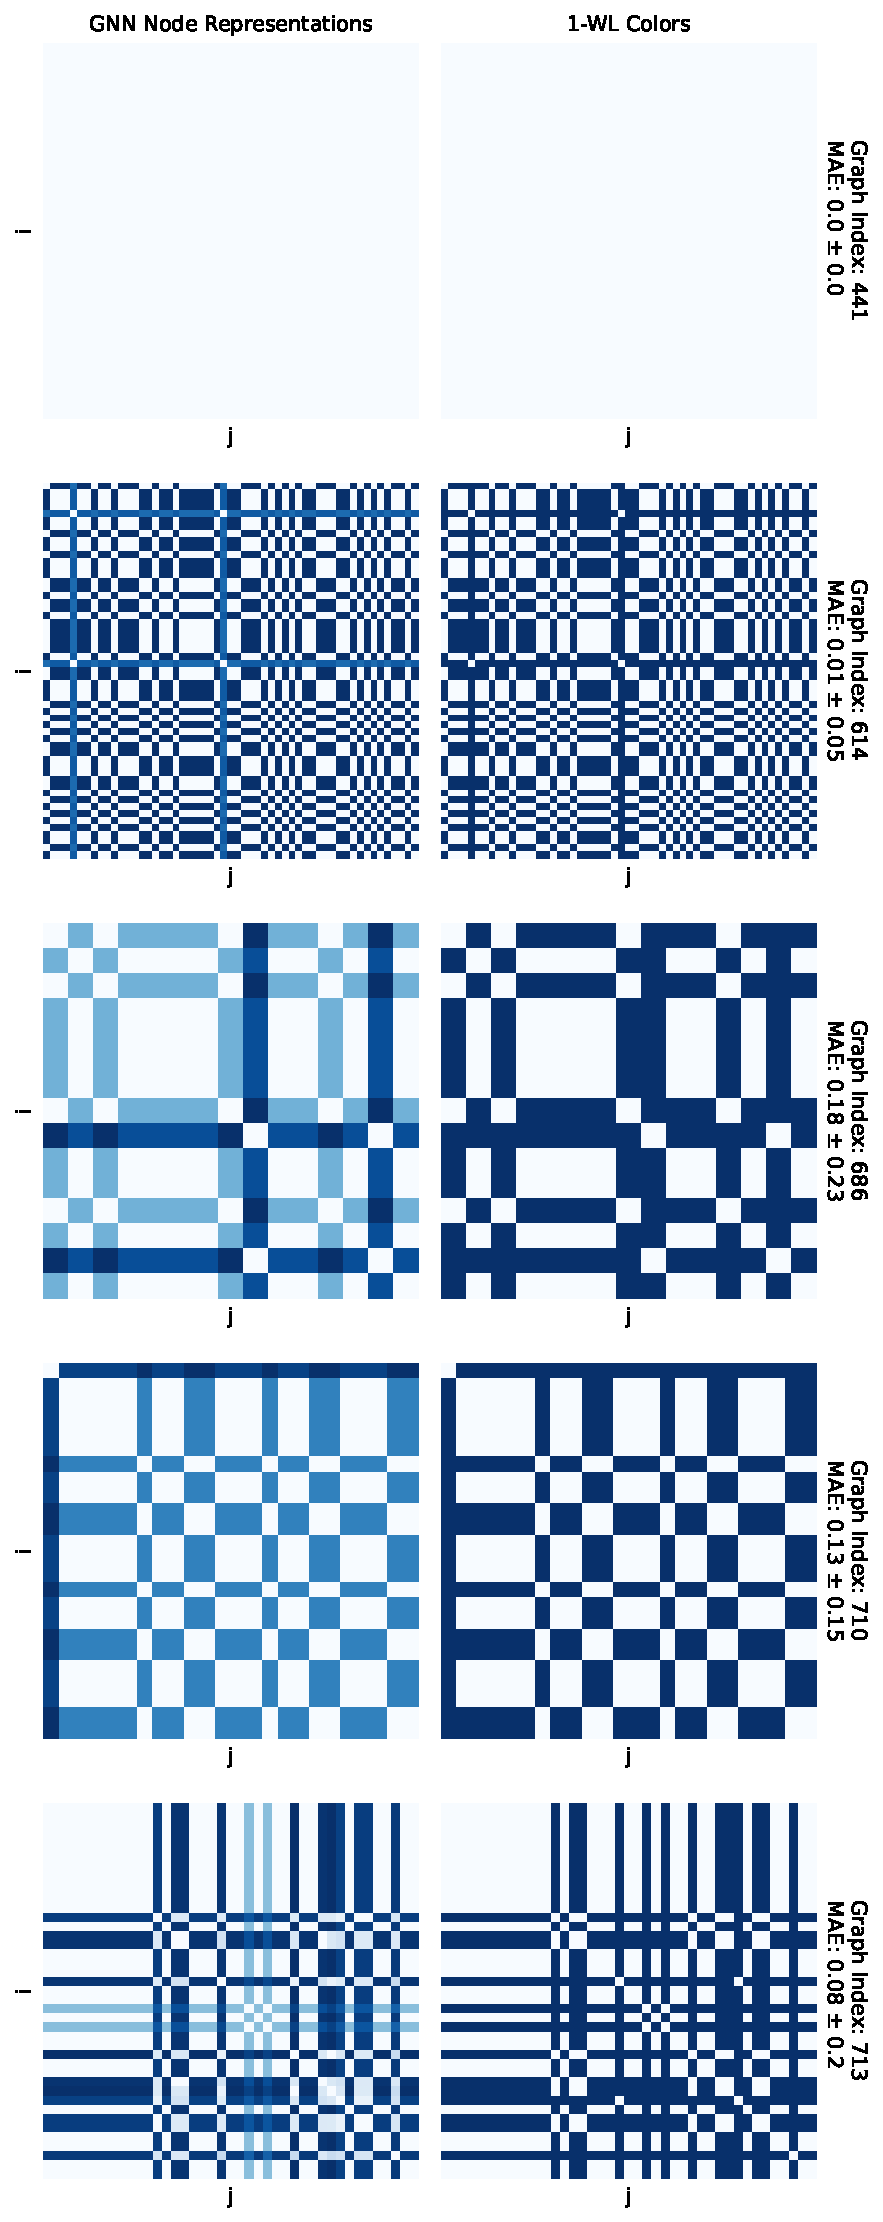
\includegraphics[width=\textwidth, left]{Figures/heatmaps_IMDB-BINARY_0.pdf}
    \end{minipage}
    \hfill
    \begin{minipage}[b]{0.53007147296\textwidth}
        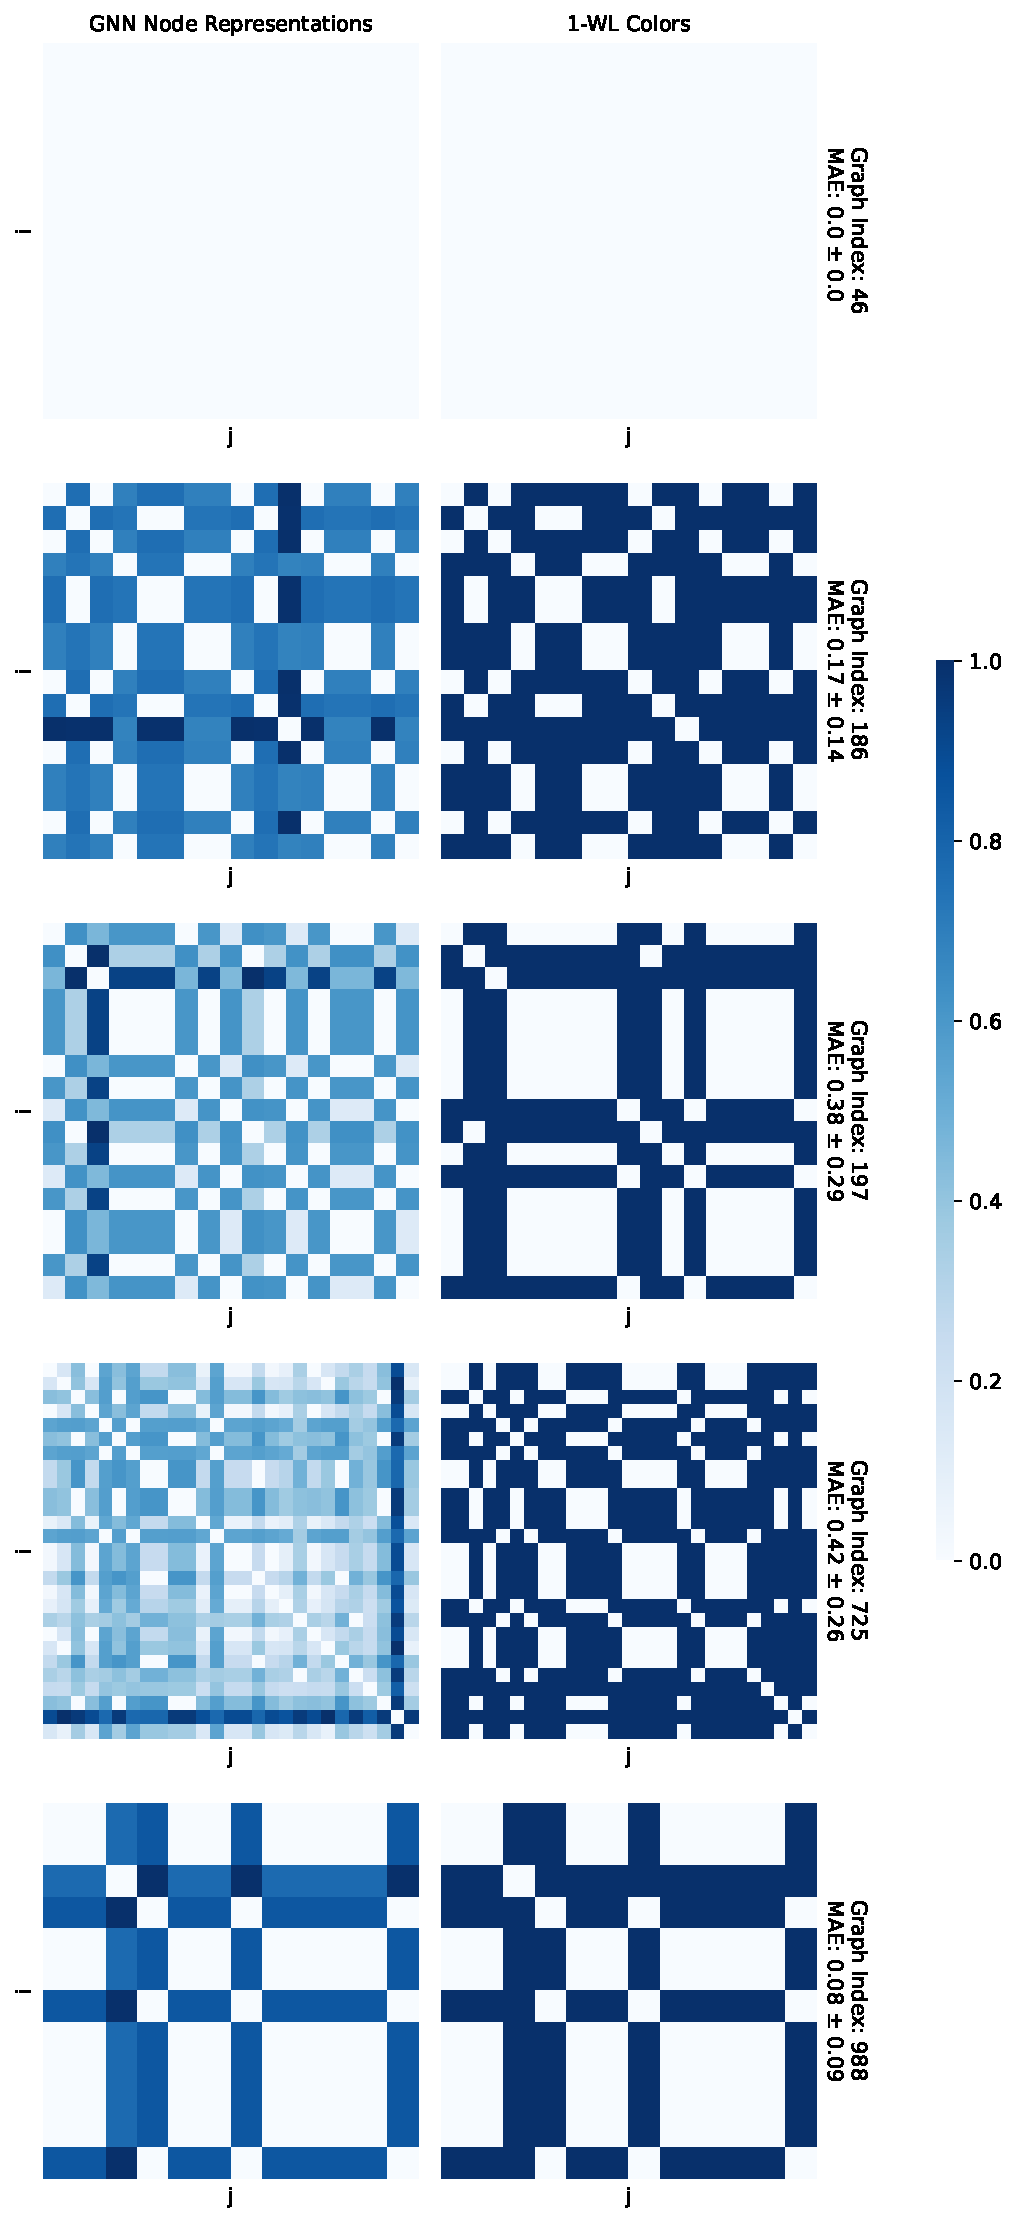
\includegraphics[width=\textwidth, right]{Figures/heatmaps_IMDB-BINARY_1.pdf}
    \end{minipage}
    \hfill
    \caption{Visualizing the performance of the best performing GNN on the \textsc{Imdb-Binary} dataset in approximating node colors computed by the 1-WL algorithm. The ten graphs shown are randomly sampled from the GNN's test set, and the 1-WL algorithm ran only for one iteration. The average error for the entire test set is $0.14 \pm 0.15$. \newline
    Note that \textsc{Imdb binary} does not contain any node features, so we artificially initialize each node feature with a one-hot encoding of its degree.}
    \label{fig:gnn_approx_imdb}
\end{figure}

\begin{figure}[!ht]
    \centering
    \begin{subfigure}[b]{0.45992852703\textwidth}
        \centering
        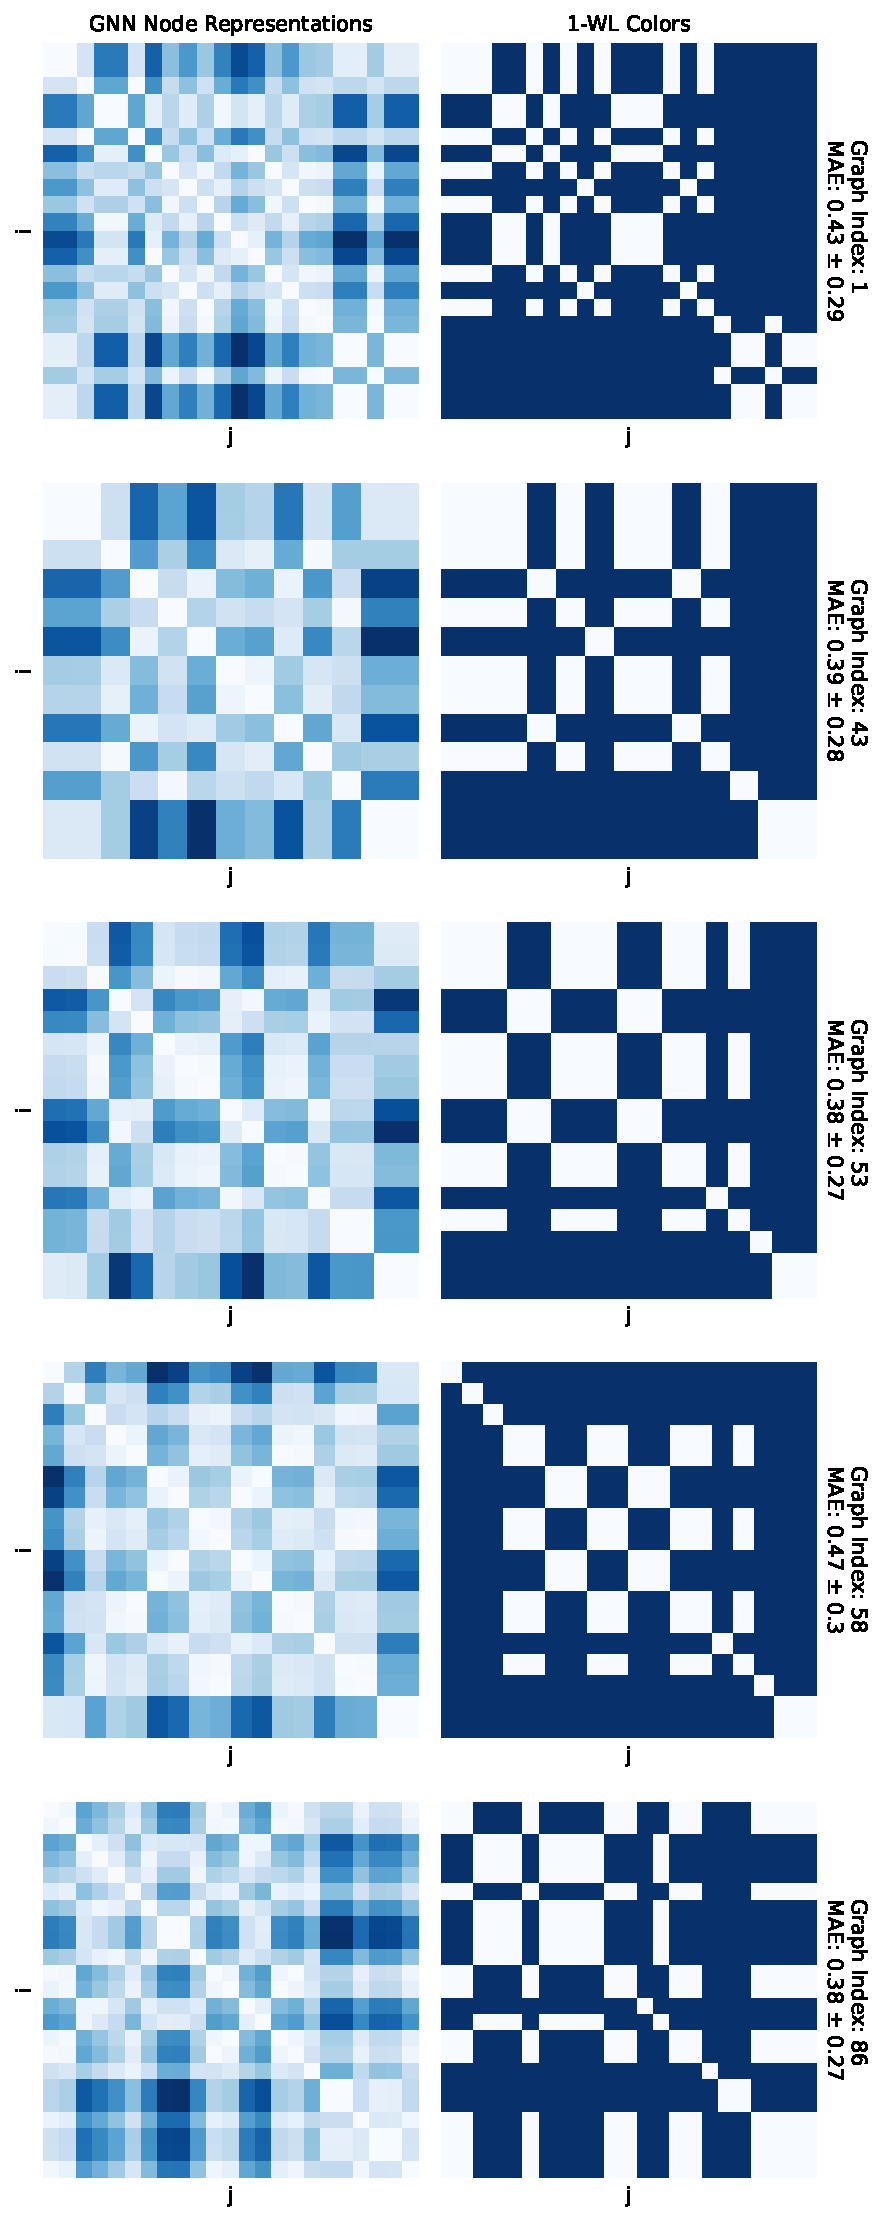
\includegraphics[width=\textwidth, left]{Figures/heatmaps_MUTAG_0.pdf}
    \end{subfigure}
    \hfill
    \begin{subfigure}[b]{0.53007147296\textwidth}
        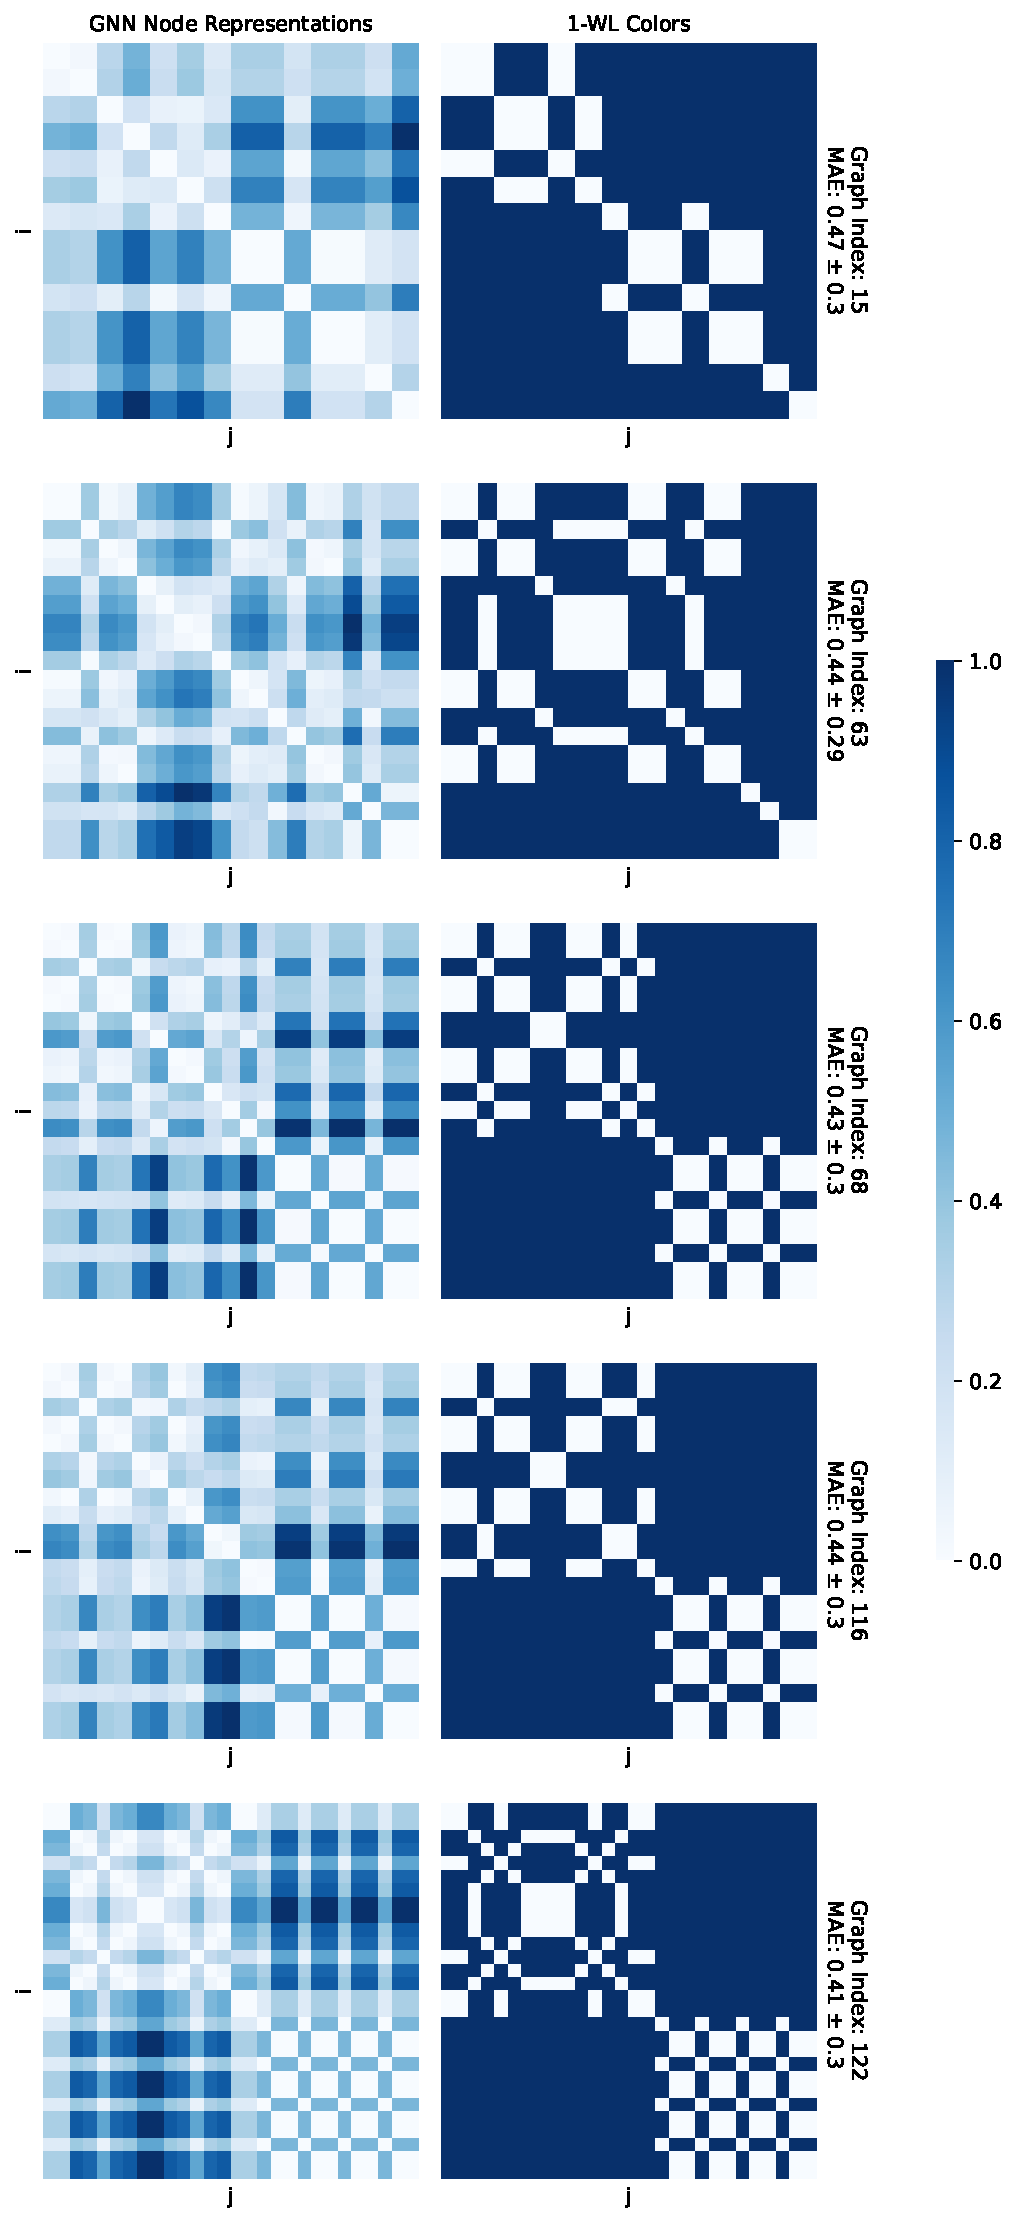
\includegraphics[width=\textwidth, right]{Figures/heatmaps_MUTAG_1.pdf}
    \end{subfigure}
    \hfill
    \caption{Visualizing the performance of the best performing GNN on the \textsc{Mutag} dataset in approximating node colors computed by the 1-WL algorithm. The ten graphs shown are randomly sampled from the GNN's test set, and the 1-WL algorithm ran only for three iteration. The average error for the entire test set is $0.42 \pm 0.29$.}
    \label{fig:gnn_approx_mutag}
\end{figure}

\begin{figure}[!ht]
    \centering
    \begin{minipage}[b]{0.45992852703\textwidth}
        \centering
        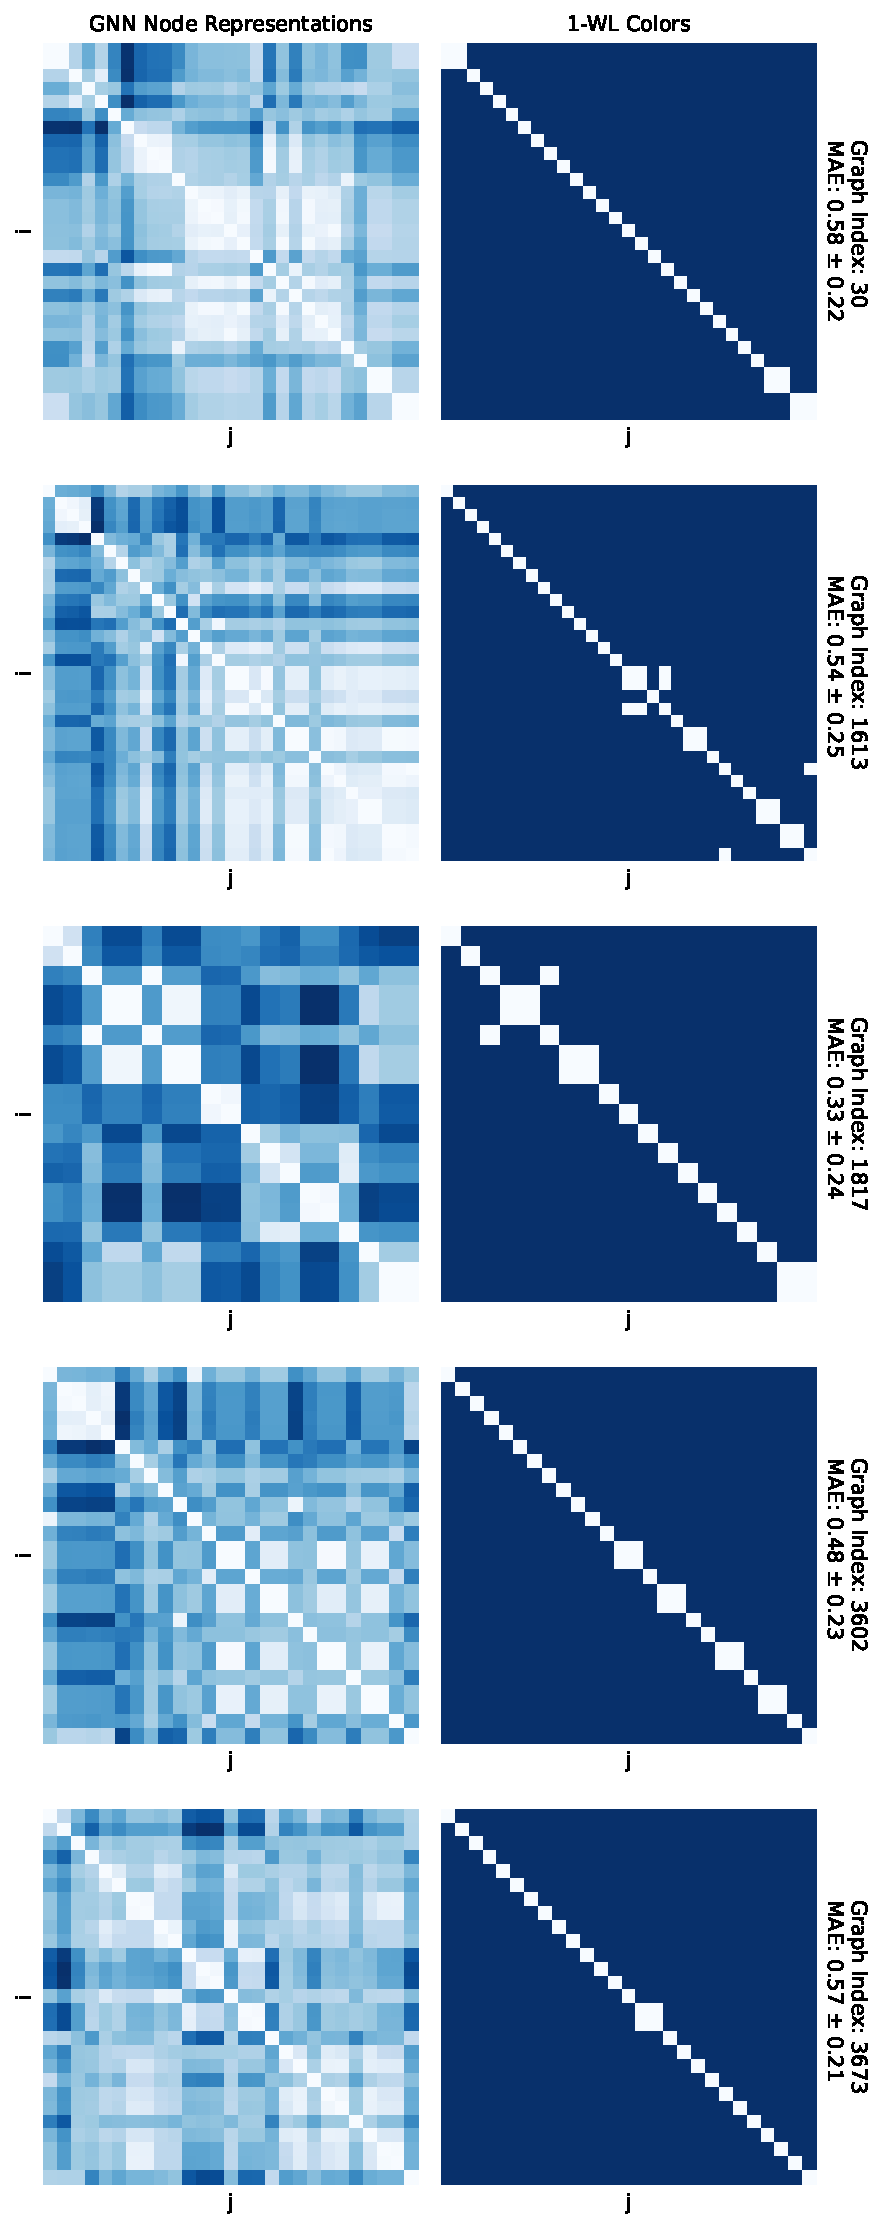
\includegraphics[width=\textwidth, left]{Figures/heatmaps_NCI1_0.pdf}
    \end{minipage}
    \hfill
    \begin{minipage}[b]{0.53007147296\textwidth}
        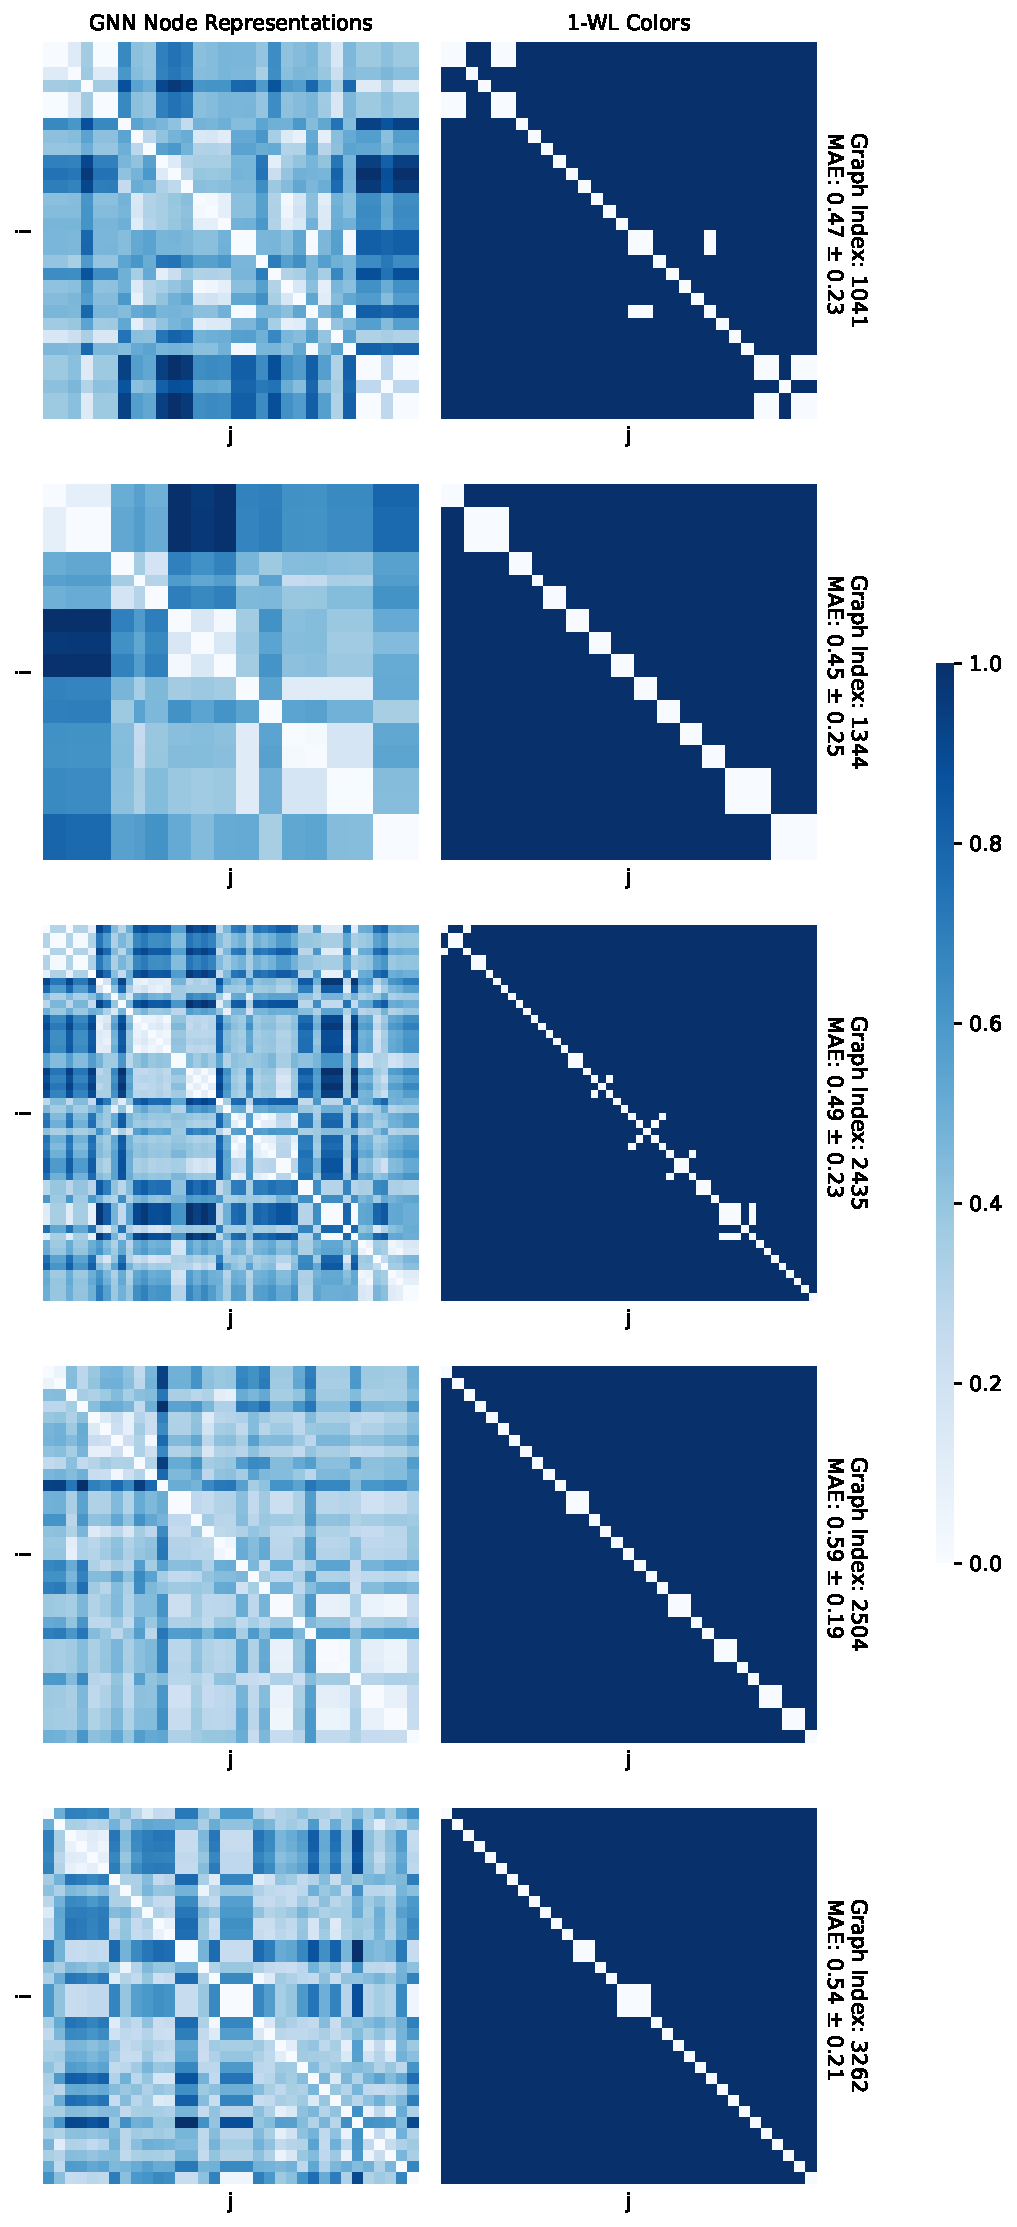
\includegraphics[width=\textwidth, right]{Figures/heatmaps_NCI1_1.pdf}
    \end{minipage}
    \hfill
    \caption{Visualizing the performance of the best performing GNN on the \textsc{Nci1} dataset in approximating node colors computed by the 1-WL algorithm. The ten graphs shown are randomly sampled from the GNN's test set, and the 1-WL algorithm ran only for three iteration. The average error for the entire test set is $0.50 \pm 0.24$.}
    \label{fig:gnn_approx_nci_3}
\end{figure}

\begin{figure}[!ht]
    \centering
    \begin{minipage}[b]{0.45992852703\textwidth}
        \centering
        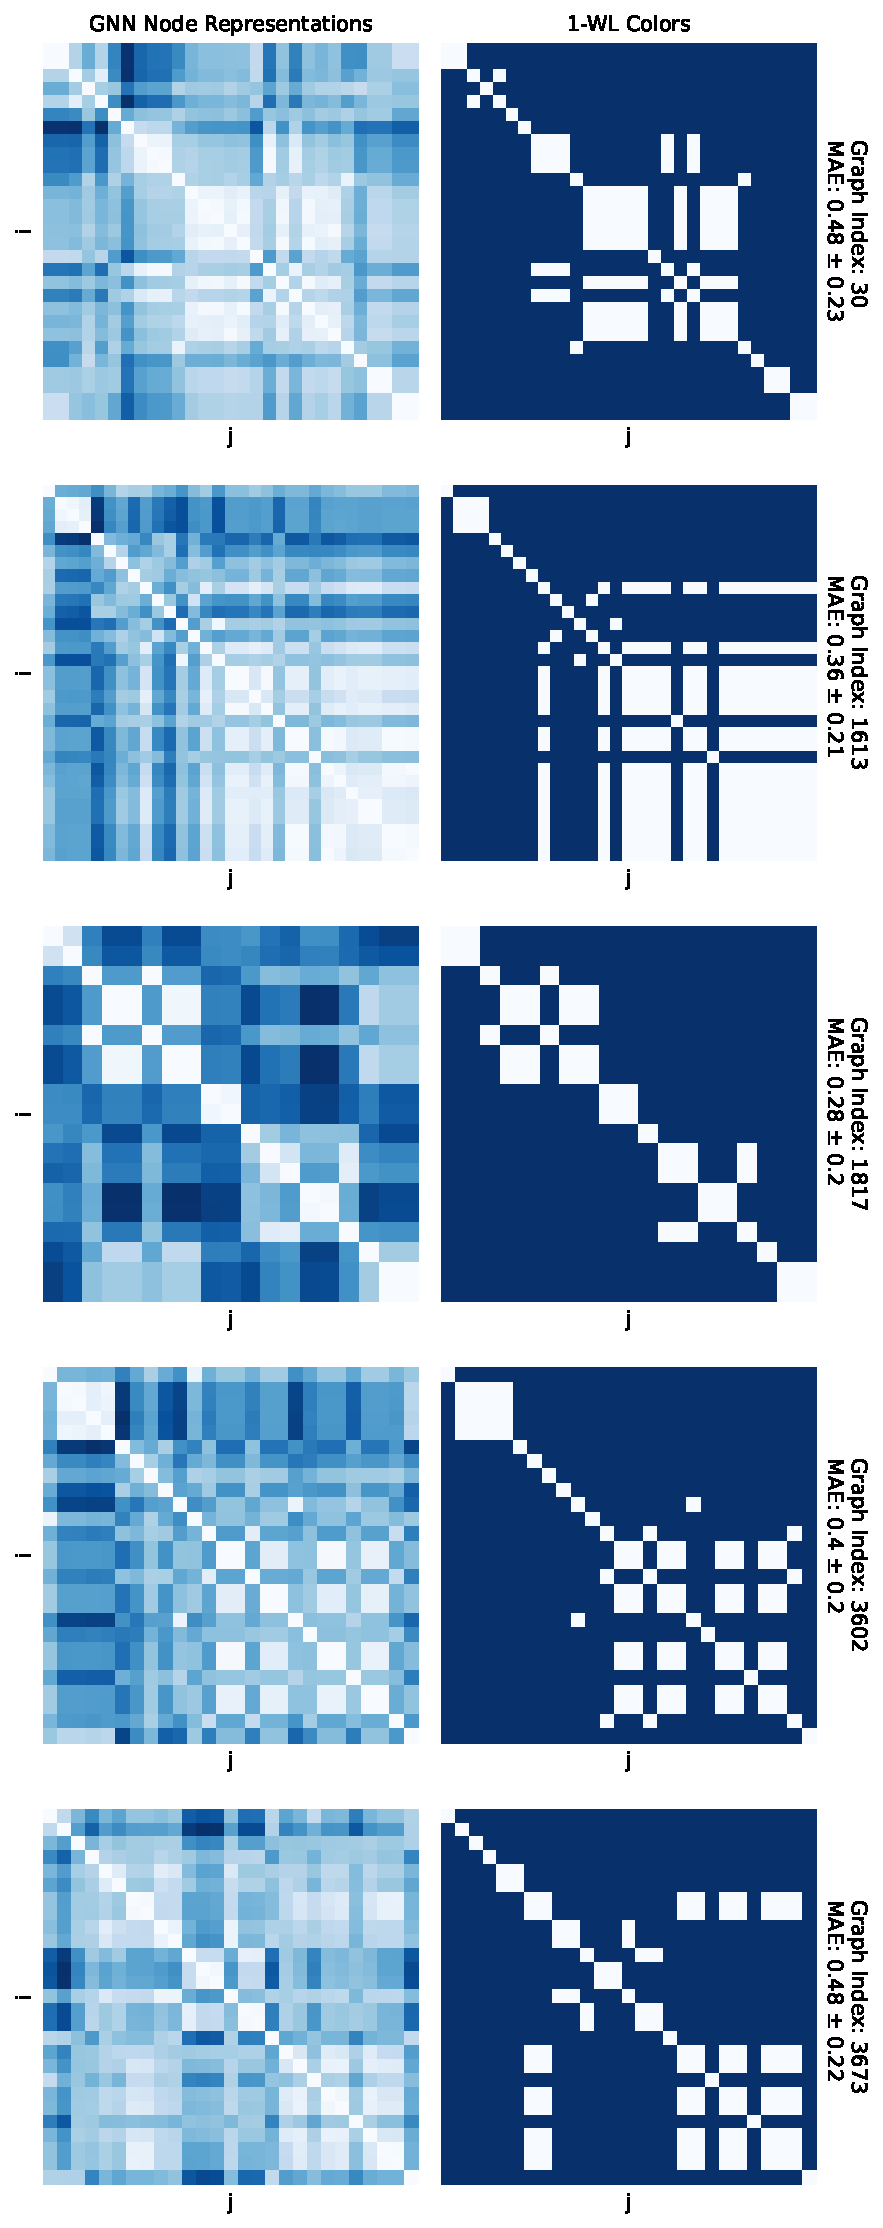
\includegraphics[width=\textwidth, left]{Figures/heatmaps_NCI1_0_k_wl_1.pdf}
    \end{minipage}
    \hfill
    \begin{minipage}[b]{0.53007147296\textwidth}
        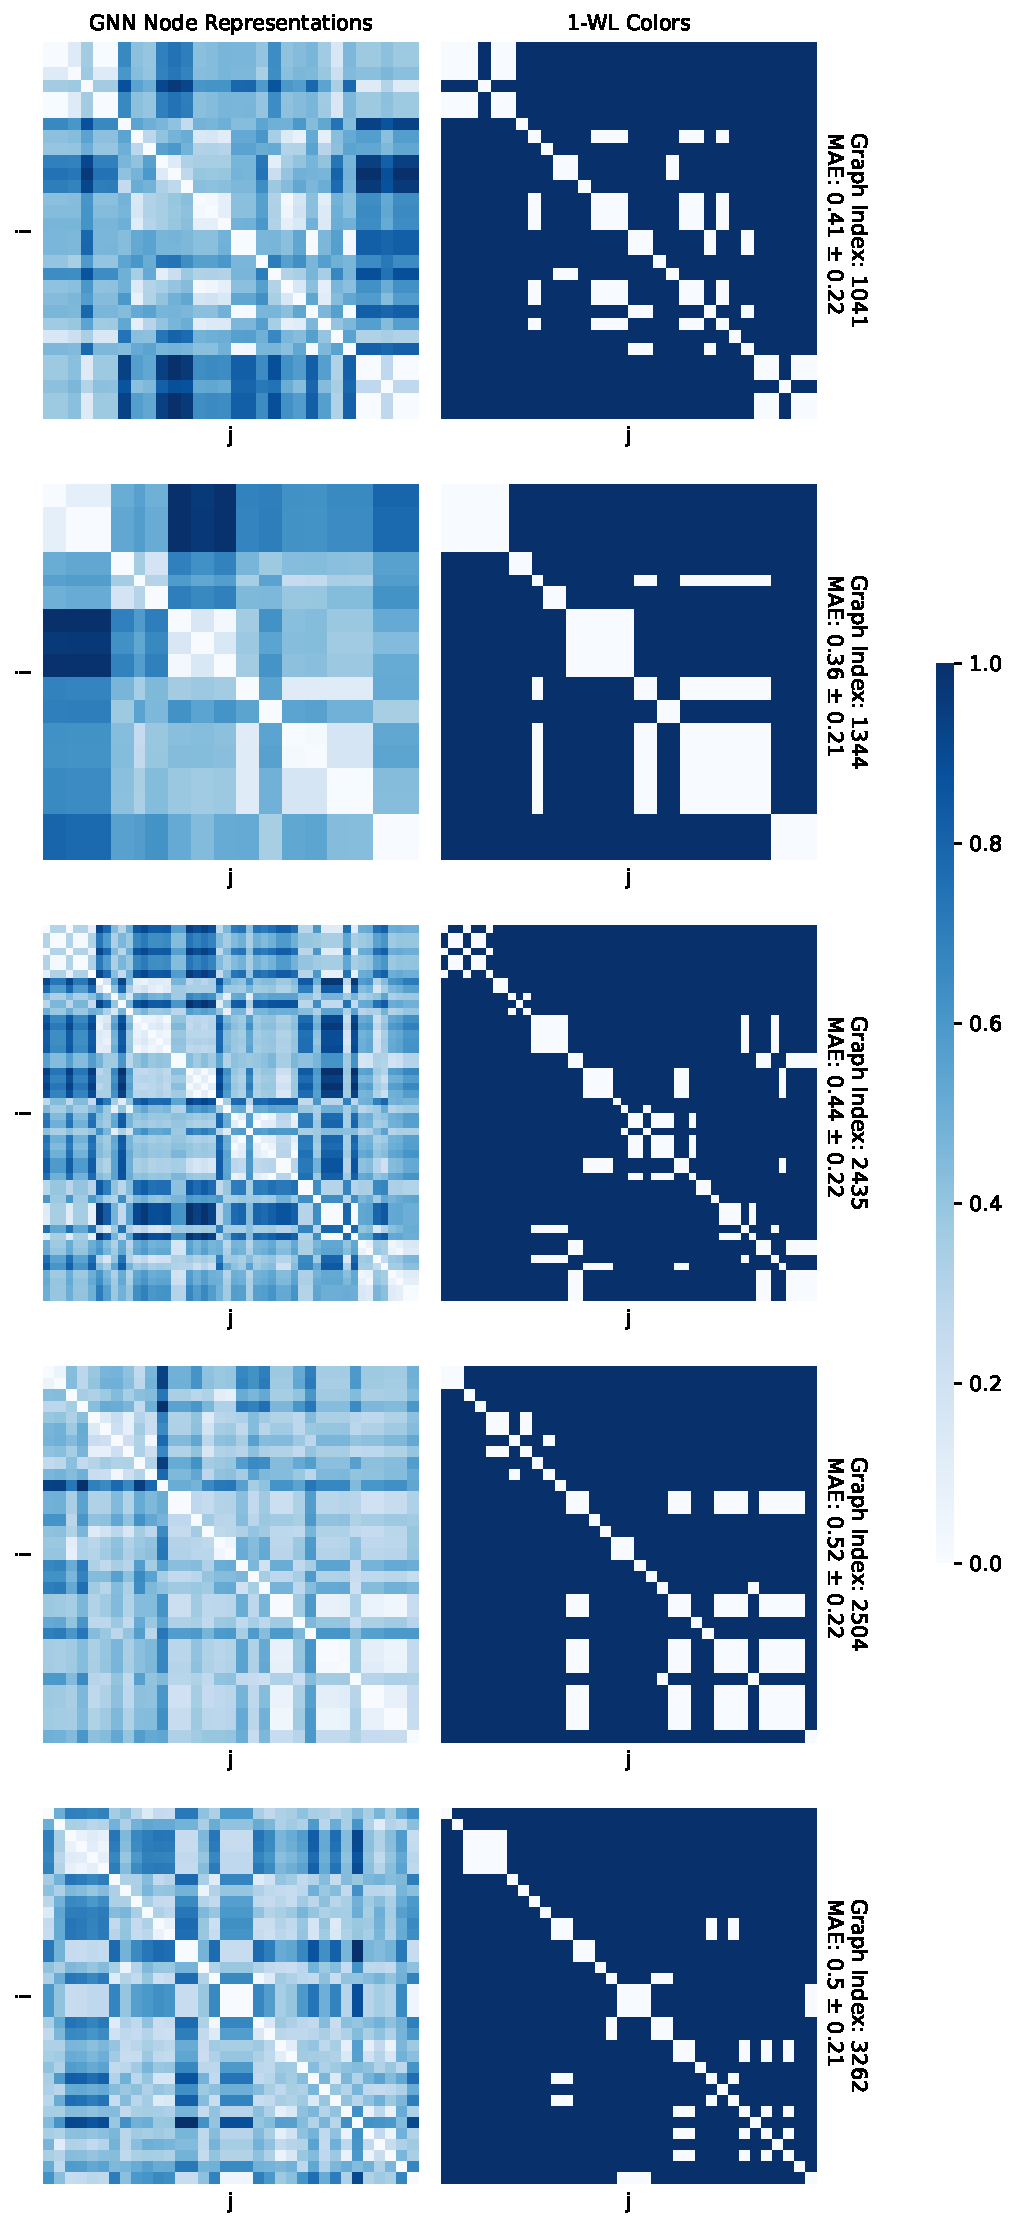
\includegraphics[width=\textwidth, right]{Figures/heatmaps_NCI1_1_k_wl_1.pdf}
    \end{minipage}
    \hfill
    \caption{Visualizing the performance of the best performing GNN on the \textsc{Nci1} dataset in approximating node colors computed by the 1-WL algorithm. The ten graphs shown are randomly sampled from the GNN's test set, and the 1-WL algorithm ran only for one iteration. The average error for the entire test set is $0.42 \pm 0.22$.}
    \label{fig:gnn_approx_nci_1}
\end{figure}

\begin{figure}[!ht]
    \centering
    \begin{minipage}[b]{0.45992852703\textwidth}
        \centering
        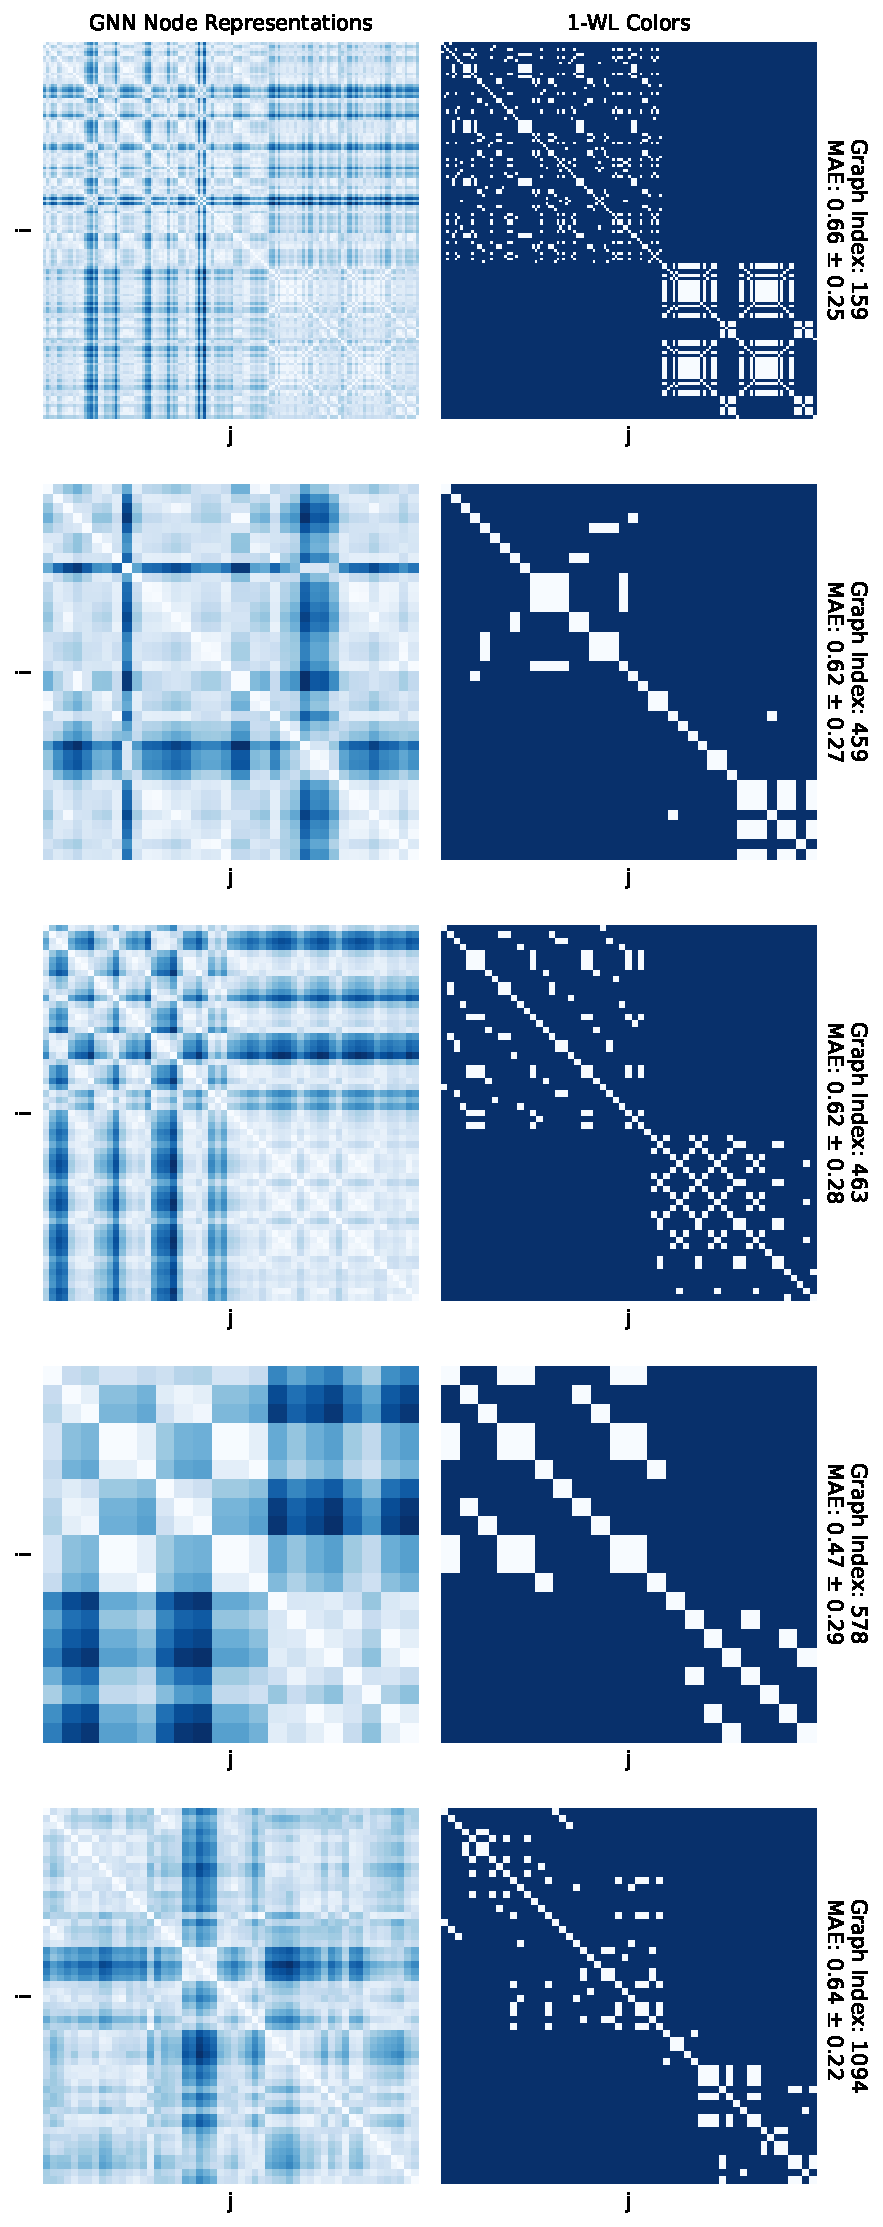
\includegraphics[width=\textwidth, left]{Figures/heatmaps_PROTEINS_0.pdf}
    \end{minipage}
    \hfill
    \begin{minipage}[b]{0.53007147296\textwidth}
        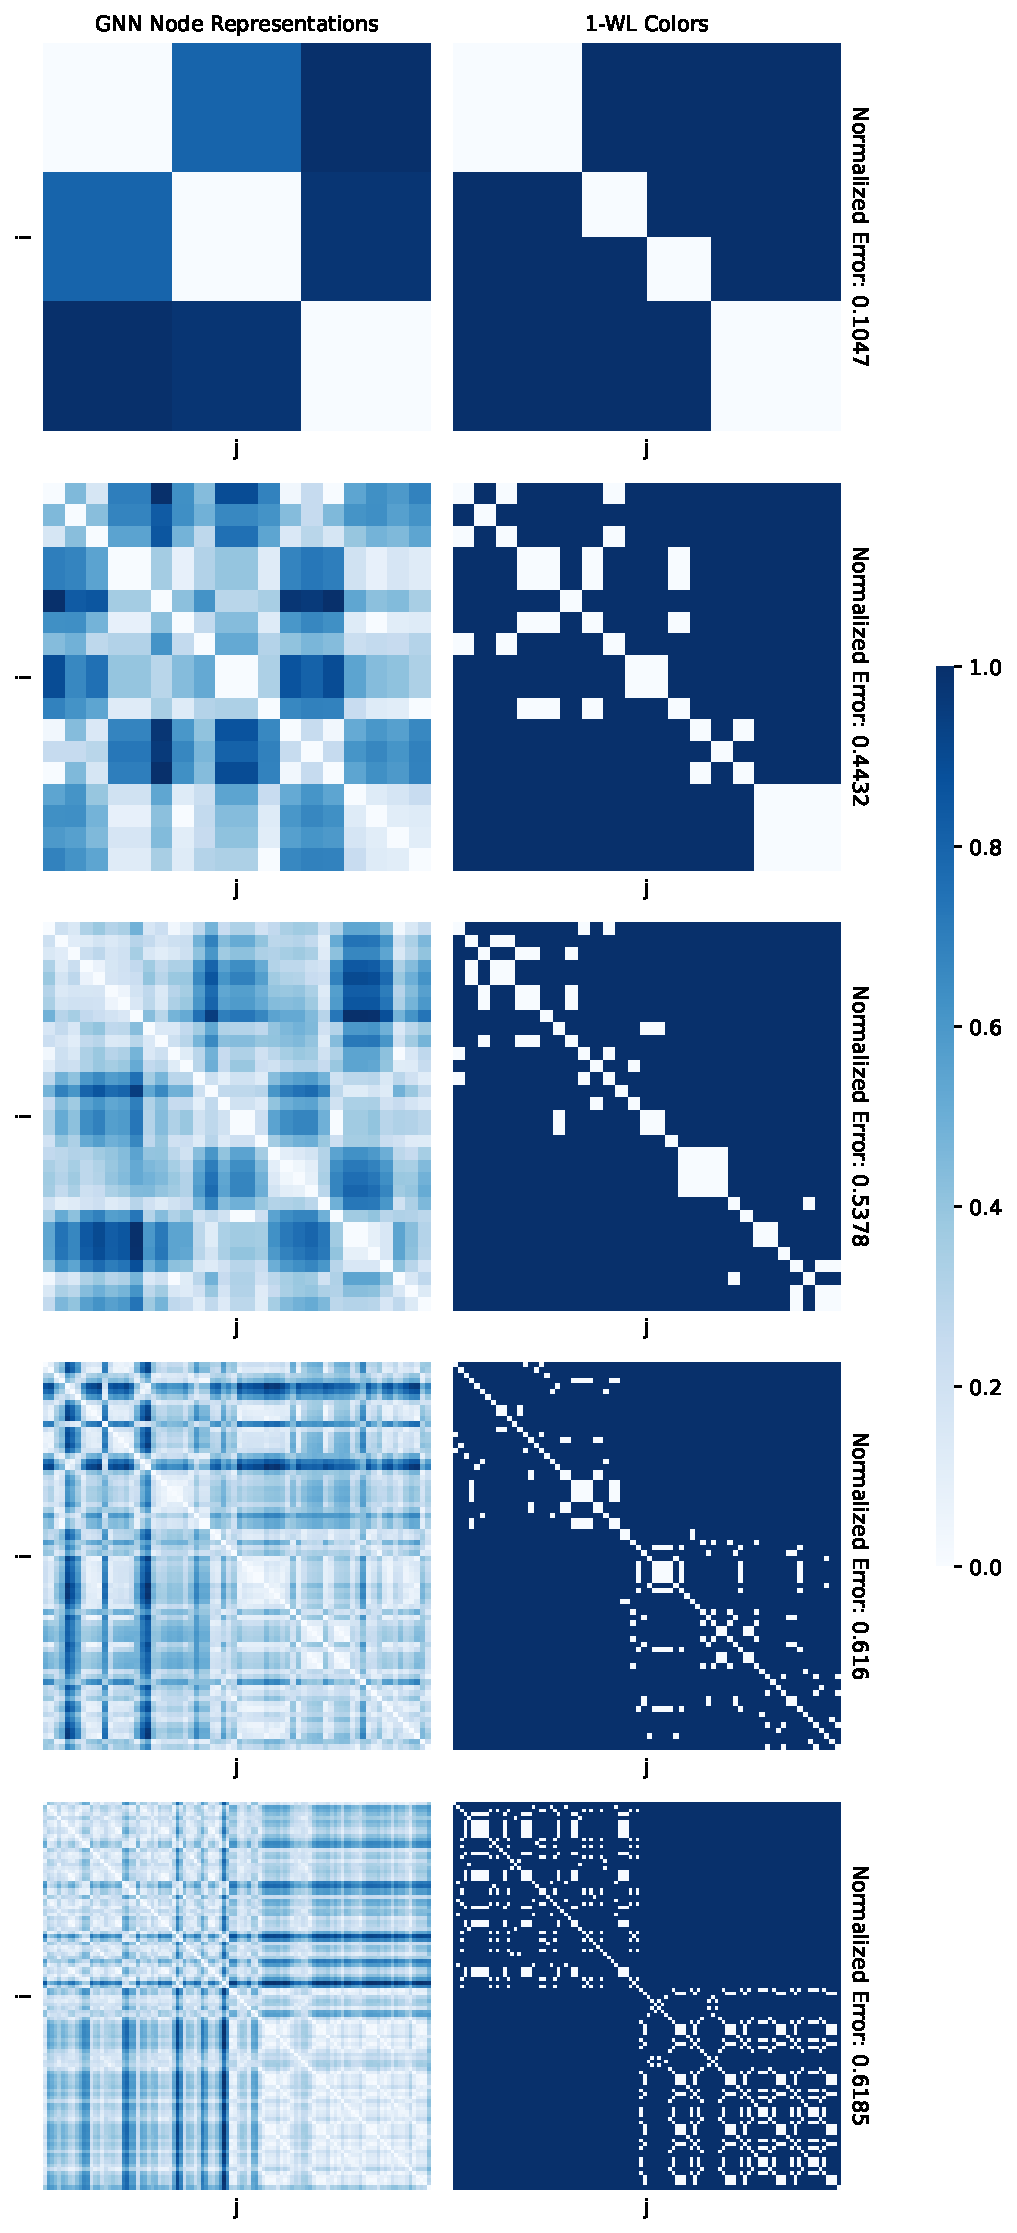
\includegraphics[width=\textwidth, right]{Figures/heatmaps_PROTEINS_1.pdf}
    \end{minipage}
    \hfill
    \caption{Visualizing the performance of the best performing GNN on the \textsc{Proteins} dataset in approximating node colors computed by the 1-WL algorithm. The ten graphs shown are randomly sampled from the GNN's test set, and the 1-WL algorithm ran only for one iteration. The average error for the entire test set is $0.49 \pm 0.26$.}
    \label{fig:gnn_approx_proteins}
\end{figure}

\begin{figure}[!ht]
    \centering
    \begin{minipage}[b]{0.45992852703\textwidth}
        \centering
        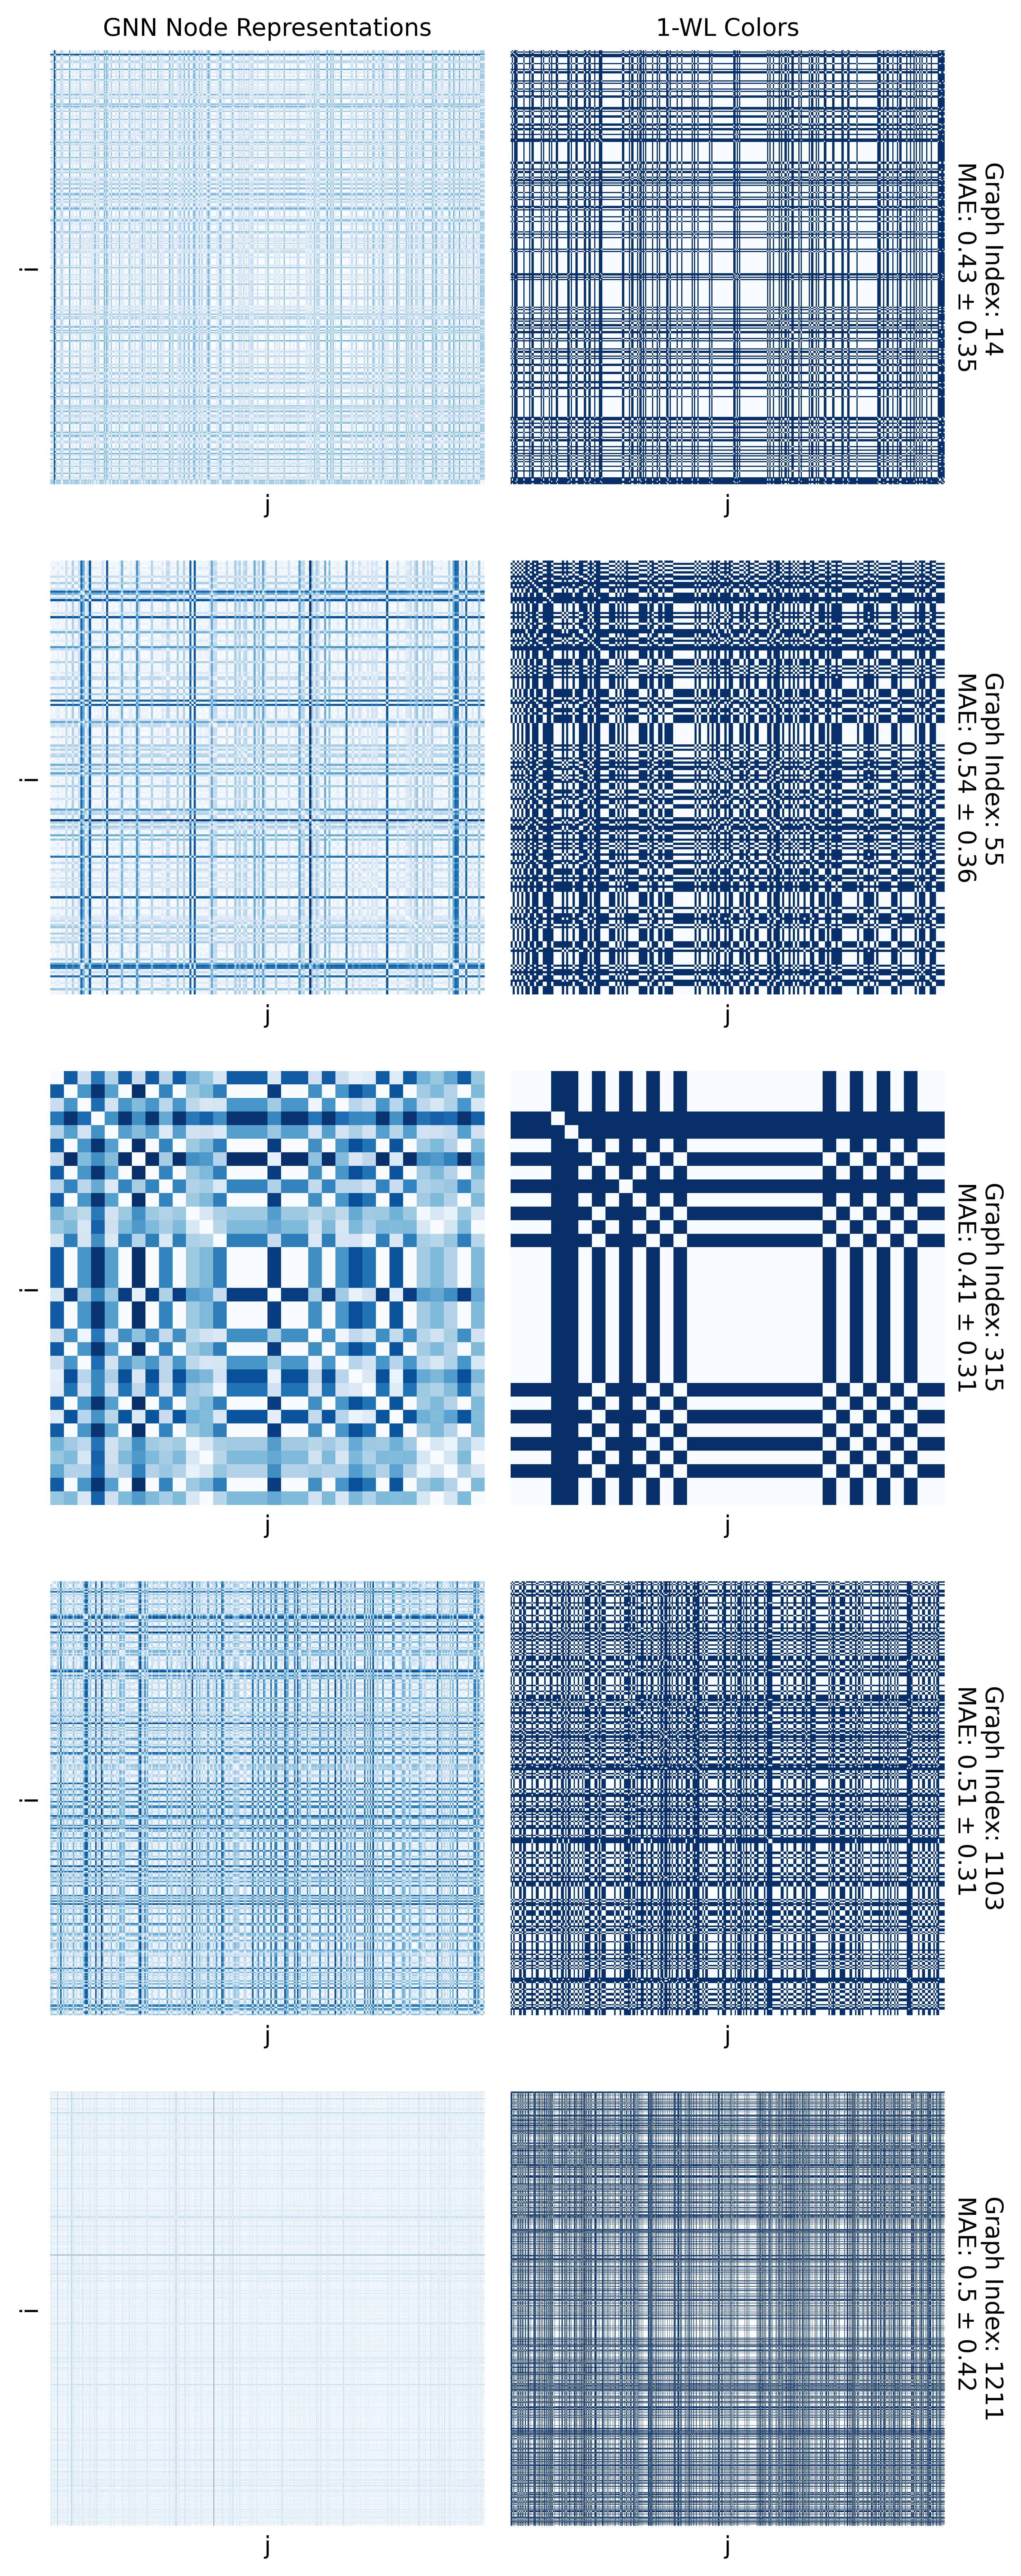
\includegraphics[width=\textwidth, left]{Figures/heatmaps_REDDIT-BINARY_0.png}
    \end{minipage}
    \hfill
    \begin{minipage}[b]{0.53007147296\textwidth}
        \includegraphics[width=\textwidth, right]{Figures/heatmaps_REDDIT-BINARY_1.png}
    \end{minipage}
    \hfill
    \caption{Visualizing the performance of the best performing GNN on the \reddit dataset in approximating node colors computed by the 1-WL algorithm. The ten graphs shown are randomly sampled from the GNN's test set, and the 1-WL algorithm ran only for one iteration. The average error for the entire test set is $0.48 \pm 0.32$.}
    \label{fig:gnn_approx_reddit}
\end{figure}